\documentclass[preprint, 3p,
authoryear]{elsarticle} %review=doublespace preprint=single 5p=2 column
%%% Begin My package additions %%%%%%%%%%%%%%%%%%%

\usepackage[hyphens]{url}

  \journal{Transport Geography?} % Sets Journal name

\usepackage{graphicx}
%%%%%%%%%%%%%%%% end my additions to header

\usepackage[T1]{fontenc}
\usepackage{lmodern}
\usepackage{amssymb,amsmath}
% TODO: Currently lineno needs to be loaded after amsmath because of conflict
% https://github.com/latex-lineno/lineno/issues/5
\usepackage{lineno} % add
\usepackage{ifxetex,ifluatex}
\usepackage{fixltx2e} % provides \textsubscript
% use upquote if available, for straight quotes in verbatim environments
\IfFileExists{upquote.sty}{\usepackage{upquote}}{}
\ifnum 0\ifxetex 1\fi\ifluatex 1\fi=0 % if pdftex
  \usepackage[utf8]{inputenc}
\else % if luatex or xelatex
  \usepackage{fontspec}
  \ifxetex
    \usepackage{xltxtra,xunicode}
  \fi
  \defaultfontfeatures{Mapping=tex-text,Scale=MatchLowercase}
  \newcommand{\euro}{€}
\fi
% use microtype if available
\IfFileExists{microtype.sty}{\usepackage{microtype}}{}
\usepackage[]{natbib}
\bibliographystyle{plainnat}

\usepackage{graphicx}
\ifxetex
  \usepackage[setpagesize=false, % page size defined by xetex
              unicode=false, % unicode breaks when used with xetex
              xetex]{hyperref}
\else
  \usepackage[unicode=true]{hyperref}
\fi
\hypersetup{breaklinks=true,
            bookmarks=true,
            pdfauthor={},
            pdftitle={Social needs for transport and gaps in transit service: new GTFS tools},
            colorlinks=false,
            urlcolor=blue,
            linkcolor=magenta,
            pdfborder={0 0 0}}

\setcounter{secnumdepth}{5}
% Pandoc toggle for numbering sections (defaults to be off)


% tightlist command for lists without linebreak
\providecommand{\tightlist}{%
  \setlength{\itemsep}{0pt}\setlength{\parskip}{0pt}}

% From pandoc table feature
\usepackage{longtable,booktabs,array}
\usepackage{calc} % for calculating minipage widths
% Correct order of tables after \paragraph or \subparagraph
\usepackage{etoolbox}
\makeatletter
\patchcmd\longtable{\par}{\if@noskipsec\mbox{}\fi\par}{}{}
\makeatother
% Allow footnotes in longtable head/foot
\IfFileExists{footnotehyper.sty}{\usepackage{footnotehyper}}{\usepackage{footnote}}
\makesavenoteenv{longtable}



\usepackage{subfig}
\usepackage{booktabs}
\usepackage{longtable}
\usepackage{array}
\usepackage{multirow}
\usepackage{wrapfig}
\usepackage{float}
\usepackage{colortbl}
\usepackage{pdflscape}
\usepackage{tabu}
\usepackage{threeparttable}
\usepackage{threeparttablex}
\usepackage[normalem]{ulem}
\usepackage{makecell}
\usepackage{xcolor}



\begin{document}


\begin{frontmatter}

  \title{Social needs for transport and gaps in transit service: new
GTFS tools}
    \author[Public Transport Research Group (PTRG)]{James Reynolds%
  %
  \fnref{1}}
   \ead{james.reynolds@monash.edu} 
    \author[Public Transport Research Group (PTRG)]{Graham Currie%
  \corref{cor1}%
  \fnref{2}}
   \ead{graham.currie@monash.edu} 
    \author[Public Transport Research Group (PTRG)]{Yanda Qu%
  %
  \fnref{3}}
   \ead{yanda.qu@monash.edu} 
      \affiliation[Public Transport Research Group (PTRG)]{
    organization={Public Transport Research Group (PTRG), Institute of
Transport Studies, Department of Civil Engineering Engineering, Monash
University},addressline={Clayton
Campus},city={Melbourne},postcode={3800},state={Victoria},country={Australia},}
    \cortext[cor1]{Corresponding author}
    \fntext[1]{Research Fellow}
    \fntext[2]{Professor}
    \fntext[3]{PhD Student}
  
  \begin{abstract}
  This is the abstract.

  It consists of two paragraphs.
  \end{abstract}
    \begin{keyword}
    keyword1 \sep 
    keyword2
  \end{keyword}
  
 \end{frontmatter}

\hypertarget{introduction}{%
\section{Introduction}\label{introduction}}

An important role for transit in many locations is to provide at least a
basic level of service, so that those who cannot otherwise drive
themselves have at least some mobility and accessibility to activities
and service beyond walking distance \citep{Currie:2016aa}. There is
evidence that a lower proportion of younger people are obtaining a
driving license than was the case previously \citep{delbosc2013causes}.
As well, age, disability, socio-economic status, lack of a vehicle or
many other factors might make someone reliant on transit for some or all
of their travel. Vertical social-equity perspectives on transport
policy-making, relating to supporting those who are disadvantaged (c.f.
\citet{Litman:2016aa}), might therefore suggest providing at least some
transit, and probably more than just a minimum, where there are higher
social needs for transport.

\citet{Currie2003Hobart}, \citet{Currie2004Gap};
\citet{Currie2007Identifying} and \citet{currie2010identifying}
developed an approach for identifying spatial gaps in transit supply
related to social needs for transport, and applied it to a case study of
Melbourne in 2006. This was suggested as being ``substantially more
useful than the presentation of anecdotal evidence, which is the most
common means of identifying transport needs in local transport studies
throughout the world'' \citep{currie2010identifying}. However, there
does not appear to have been much further use or development of this
spatial analysis technique. It is unclear whether the geographic
patterns identified in this previous research are representative of
transit supply and social needs in other places, or if the situation in
Melbourne has changed in the intervening years. This may in part be
because until recently schedules was not typically available in
consistent and electronic formats, meaning that assessing transit supply
was a large task requiring bespoke sourcing, cleaning and analysis of
data for each transit operator.

Nowadays, however, more than 10,000 transit agencies publicly release
timetable data in the General Transit Feed Specification (GTFS) format
\citep{GTFS}. Such standardisation allows Google Maps and other online
platforms to provide transit-related outputs for any place publishing a
feed. It also facilitates data access and processing for research
purporses. However, tools for using GTFS data to examine spatial
patterns and gaps in transit supply with respect to social needs for
transport do not appear to be readily available. This gap, and the lack
of direct follow up to \citet{Currie2003Hobart}, \citet{Currie2004Gap},
\citet{Currie2007Identifying} and \citet{currie2010identifying}, provide
motivation for this research.

The objectives of this research are: (1) to develop tools for
undertaking needs-gap analysis using GTFS datasets; and (2) to explore
whether the spatial pattern of gaps reported in
\citet{Currie2007Identifying} and \citet{currie2010identifying} are
consistent with current patterns. Research outcomes that are reported in
this paper include the development of a new R package (gtfssupplyindex)
that includes software tools for using the \citet{Currie2007Identifying}
and \citet{currie2010identifying} analysis approach, in particular the
calculation of transit Supply Index (SI) scores from GTFS datasets. Also
presented in this paper are results for Melbourne in 2016 and 2021,
matching the most recent censuses, for comparison to the 2006 results
reported in \citet{currie2010identifying}\footnote{The wider programme
  of research includes examination of spatial gaps in other cities, so
  as to better understand whether patterns in Melbourne are
  representative of other places. However, this paper is limited to
  examining Melbourne in 2016 and 2021 only. Results for other cities
  will be reported elsewhere.}.

The remainder of this paper is structured as follows: the next section
outlines the research context. Section 3 describes the study
methodology, followed by presentation of results in Section 4 and
discussion in Section 5. Limitations of this study and directions for
future research are discussed in Section 6, which concludes the paper.

\hypertarget{research-context}{%
\section{Research context}\label{research-context}}

There are many metrics available for assessing transit services.
Examples include: those in the \emph{Transit Cooperative Research
Program (TCRP) Report 88: a guidebook for developing
performance-measurement systems} \citep{Ryus:2003aa}; and those used
across benchmarking databases and programs such as by
\citet{Florida-Transit-Information-System:2018aa}, the
\citet{UITP:2015aa} and \citet{Imperial-College-London:2023aa}. The
Fielding Triangle \citep{FieldingGordonJ1987Mpts} provides a framework
for combining indicators of service inputs, outputs and consumption to
describe cost efficiency, cost effectiveness and service effectiveness.
More broadly: \citet{Litman:2003ab} and \citet{Litman:2016aa} discuss
some of the traffic, mobility, accessibility, social equity, strategic
planning and other rational decision-making perspectives underlying many
transport indicators; \citet{Reynolds:2017ah} extends these into models
of how institutionalism, incrementalism and other public policy analysis
concepts might apply to decision-making processes relating to transit
prioritisation; \citet{GuzmanLuisA.2017Aeit} developed a measure of
accessibility in the context of policy development and social equity for
Latin American Bus Rapid Transit (BRT) networks; and
\citet{Creutzig2020streetspaceallocation} introduced street space
allocation metrics based around ten ethical principles.

Many such metrics, however, may be difficult to calculate, explain or
understand, especially for those who are not planners, engineers or
other technical specialists. Where pre-calculated transit metrics are
immediately available, such as on a website, it may not be possible to
independently generate scores and assess proposed system changes.
Contrasting examples are provided by:

\begin{itemize}
\item
  \emph{Transit Scores} \citep{WalkScore:2023tg}, which are readily
  available online for locations with a published GTFS feed. The meaning
  of the metric appears easy to explain, with the highest possible score
  of 100 representing the sort of transit accessibility experienced in
  the center of New York. However, the algorithm is secret, and scores
  cannot be calculated independently.
\item
  The \emph{Transit Capacity and Quality of Service Manual (TCQSM)},
  which provides a wide range of metrics for measuring different aspects
  of a transit system. The scores themselves appear easy to understand
  or explain, ranging from A (good) to F (bad), but there are many
  metrics,\\
  which may add to the complexity of using these in practice for
  communication with non-technical audiences (e.g.~the public,
  politicians or other stakeholders). TCQSM scores, however, can be
  calculated independently, given sufficient data.
\end{itemize}

The widespread availability of GTFS datasets in recent years has
facilitated the development of tools that apply one or a group of
metrics to many transit systems. The \emph{Transit Score} website
provides one example. \citet{Wong:2013aa} provides another in reporting
the distribution of various TCQSM metrics across 50 USA transit
operators. Code used in the \citet{Wong:2013aa} analysis is available
for those who might wish to produce similar analysis for other locations
or time periods. Developing a similar code base for calculating metrics
associated with spatial gaps in transit supply with respect to social
needs is an objective of the research reported in this paper.

\hypertarget{the-transit-suppy-index}{%
\subsection{The Transit Suppy Index}\label{the-transit-suppy-index}}

A generalized form of the SI equation, adapted from
\citet{currie2010identifying}, is:

\[SI_{area, time} = \sum{\frac{Area_{Bn}}{Area_{area}}SL_{n, time}}\]

where:

\begin{itemize}
\item
  \(SI_{area, time}\) is the Supply Index for the area of interest and a
  given period of time;
\item
  \(Area_{Bn}\) is the buffer area for each stop (n) within the area of
  interest (in \citet{currie2010identifying} this was based on a radius
  of 400 metres for bus and tram stops, and 800 metres for railway
  stations);
\item
  \(Area_{area}\) is the area of the area of interest; and
\item
  \(SL_{n,time}\) is the number of transit arrivals for each stop for a
  given time period.
\end{itemize}

\begin{figure}

{\centering \subfloat[Distribution of Transport Supply\label{fig:Currie_map_SI-1}]{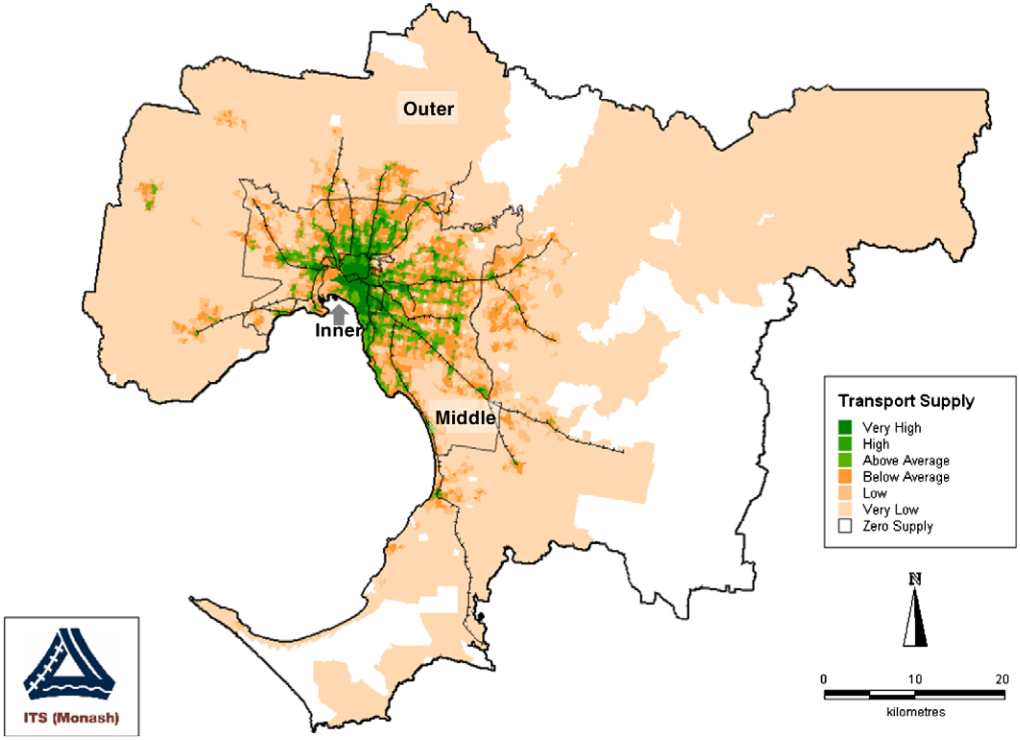
\includegraphics[width=0.5\linewidth]{graphics/Currie2010SI} }\subfloat[Distibution of Social Need for Transport\label{fig:Currie_map_SI-2}]{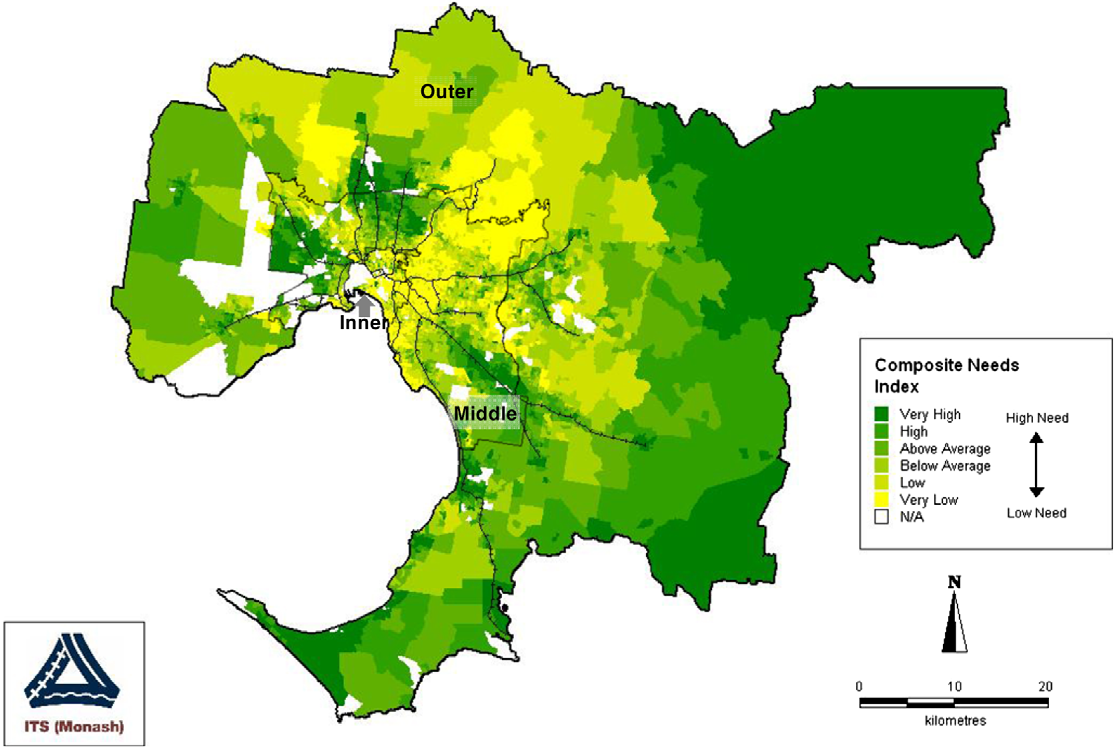
\includegraphics[width=0.5\linewidth]{graphics/Currie2010Needs} }\newline\subfloat[Supply Index and Composite Needs Index scores\label{fig:Currie_map_SI-3}]{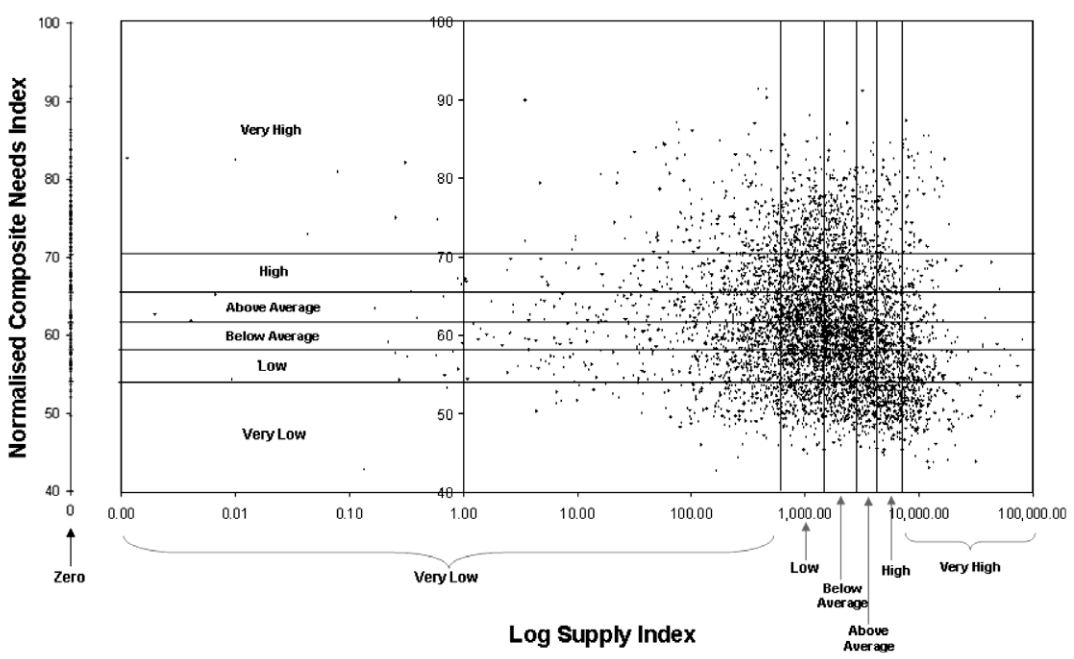
\includegraphics[width=0.5\linewidth]{graphics/Currie2010chart} }\subfloat[CCDs with Very High needs and Very Low or Zero supply\label{fig:Currie_map_SI-4}]{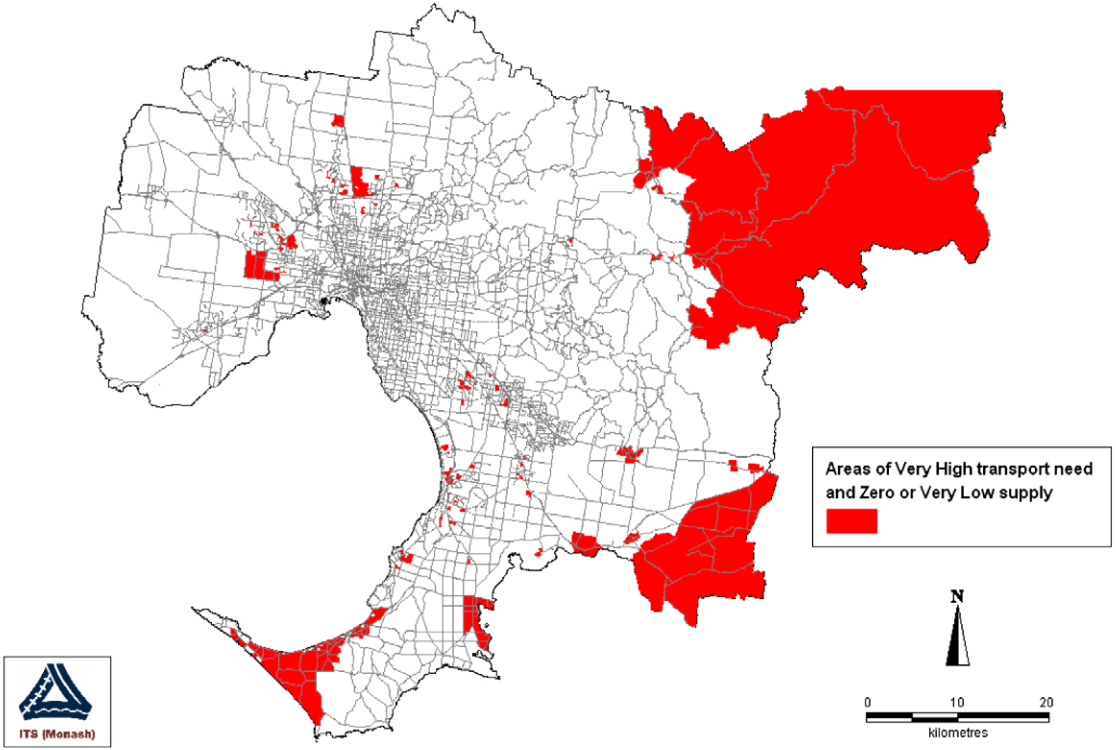
\includegraphics[width=0.5\linewidth]{graphics/Currie2010gap} }\newline

}

\caption{Melbourne 2006 Social Needs-Gap Results. Source: Currie (2010)}\label{fig:Currie_map_SI}
\end{figure}

\citet{currie2010identifying} reported SI scores for Census Collection
Districts (CCDs) across Melbourne in 2006. These were used to categorise
service levels into seven groups, as shown in Figure
\ref{fig:Currie_map_SI} (top). General patterns were identified, being:
more transit supply in the inner and middle suburbs, and along passenger
railway lines; and outer areas tending to have very low SI scores or no
transit supply at all.

\hypertarget{social-need-and-needs-gap}{%
\subsection{Social need and needs-gap}\label{social-need-and-needs-gap}}

As well as measuring transit supply, \citet{currie2010identifying}
assessed the social need for transport across Melbourne using a
composite index including: the Australian Bureau of Statistics' (ABS')
Index of Related Socio-Economic Advantage/Disadvantage (IRSAD) and a
transport needs index derived from eight weighted indicators. The
spatial distribution of this composite social needs index, reproduced in
Figure \ref{fig:Currie_map_SI} (middle), showed that areas of above
average, high and very high social needs in 2006 were located in: some
outer areas, particularly in the east and south-east; and in some middle
areas in the south-east, north and west.

As the final step in the spatial needs-gap analysis,
\citet{currie2010identifying} identified areas with very high transport
needs, but very low or zero transit supply, as reproduced in Figure
\ref{fig:Currie_map_SI} (bottom). These areas were identified as being
those where service gaps might be of particular concern. Most of these
were located in outer parts of Melbourne in the north-east, south-east
and south, although there were also some pockets in the middle suburbs
in the west, north and south east. Overall,
\citet{currie2010identifying} found that ``8.2\% of Melbourne residents
have `very high' needs but `zero', `low' or `very low' public transport
supply.''

However, it does not appear that this approach has been widely adopted
in practice or by researchers. Our suspicion is that while the SI has a
relatively simple formula and requires only geographic and timetable
data to calculate, a lack of software tools to complete the analysis may
be partly why it has not been more widely adopted. It is also unclear
whether the patterns in Melbourne identified in
\citet{currie2010identifying} have changed since the 2006 analysis, or
if Melbourne is representative of other locations. Developing a software
tool to calculate SI tools from GTFS data, and using it to comparing
current conditions to the findings of \citet{currie2010identifying},
therefore, provides motivation for this research.

\hypertarget{methodology}{%
\section{Methodology}\label{methodology}}

Case research approaches can be particularly useful when research
questions are about `how' or `why', but researchers lack control of
events (and so cannot use experimental approaches)\citep{Yin2009aa}. In
this study the research questions relate to (1) how to use GTFS data to
assess gaps between social needs and transit supply, and (2) how and why
spatial patterns might have changed since those reported for 2006 in
\citet{currie2010identifying}. There is no ability here to control
events related to the spatial patterns of social needs and gaps in
transit supply, so a case research approach appears well suited to this
study.

There is a need to address the ``duality criterion'' when using a case
research approach, this being that the study should be seeking
generalisable findings while at the same time being grounded in the
context of only a small number of cases (thereby allowing cases to be
examined in great depth)\citep{Denscombe2007aa, Ketokivi2014aa}. Here
the approach taken has been to develop a package of tools for
calculating the SI from GTFS data using the R programming language
\citep{R-base}. Using these methods addresses the duality criterion for
the first research question, as the developed software functions are
generic and might be apply to other GTFS feeds. As such they could be
used to analyse spatial gaps in transit supply in other places (and by
others), beyond the Melbourne case reported in this paper. The
recommendations of \citet{wickham2023r} informed the package setup and
development approach. Various existing packages and code examples were
relied upon including: the sf package \citep{R-sf} for geospatial
analysis; the tidyverse \citep{tidyverse2019}; gtfstools
\citep{R-gtfstools}; and tidytransit \citep{R-tidytransit}.

There are, however, limitations to the generalisability of the findings
of this research with respect to changes since 2006 and the patterns
reported in \citet{currie2010identifying}(research question 2).
\citet{Currie2007Identifying} and \citet{currie2010identifying} reported
results for Melbourne only. The \citet{Currie2003Hobart} and
\citet{Currie2004Gap} studies of Hobart and Adelaide used earlier
versions of the needs-gap assessment methodology, for which further
software tools have not been developed. While this study does seek to
findings about changes in spatial patterns of social need and transit
supply that are generalisable to more than just Melbourne, a lack of
2006 results for other cities may limit the extent to which these
findings might be confidently considered representative of changes in
other places\footnote{Other parts of this research programme will
  examine changes over the last 10-15 years in other cities (where GTFS
  data is available). The focus of this paper, however, is on Melbourne.}.

\hypertarget{code-developement}{%
\subsection{Code developement}\label{code-developement}}

Code was developed and tested on the Mornington Peninsula Tourist
Railway GTFS feed. This was selected primarily for convenience, given
that the authors are familiar with the surrounding geography and that
the feed covers only a small number of trips across just three stations
(thereby facilitating hand verification of outputs). ABS data was used
to define areas of interest, and was sourced via the absmapsdata package
\citep{absmapsdata}.

\hypertarget{melbourne-case-study}{%
\subsection{Melbourne Case Study}\label{melbourne-case-study}}

The methodological literature provides guidance on case selection and
discussion of various theoretical sampling approaches, including
sampling for critical, particularly revelatory and/or representative
cases
\citep{Eisenhardt1989aa, Yin2009aa, Denscombe2007aa, Eisenhardt2007TBfC}.
\citet{Yin2009aa} notes the selection of a case so as to allow
longitudinal study, and it is this that is the primary reason for the
selection of Melbourne for the research reported in this paper. This
selection allows direct comparison with the 2006 results reported in
\citet{currie2010identifying} so as to explore the extent to which
spatial patterns of needs-gaps in transit supply have changed over the
last 10 to 15 years. As such, SI scores were calculated using the same
Census Collection Districts (CCDs) used by
\citet{currie2010identifying}, but for the weeks starting the day of the
2016 and 2021 censuses. The Victorian GTFS feed, published by Public
Transport Victoria (PTV), was used, with historical feeds sourced from
\citet{transitfeeds_victoria:2023aa}.

Unfortunately, it is not possible to obtain 2016 or 2021 social
disadvantage data for CCDs, as the ABS no longer releases data using
this geographic scheme. Instead, population and other statistics are now
released for Statistical Area (SA1) zones, under a hierarchical
structure ranging from SA1s (\textasciitilde400 people) to SA4s (parts
of a city or region). As such, SI scores have also been calculated for
SA1s to facilitate the use of ABS data.

The same Transport Supply categorizations have been used as in
\citet{currie2010identifying} (Zero, Very Low, Low, Below average, Above
average, High and Very High). As well, this study adopts a similar
approach to measuring social disadvantage as used in
\citet{currie2010identifying}, using: the ABS' IRSAD and a transport
needs index\footnote{The same need indicators and weightings used in
  \citet{currie2010identifying} were adopted, although \$799 or lower
  per week was used as the threshold for low income households rather
  than \$499 to account for inflation (as per the Reserve Bank of
  Australia's online inflation calculator).}. A composite needs
indicator was derived based on the IRSAD and the transport needs index,
again as per the \citet{currie2010identifying} approach. However,
changes to the ABS reporting systems meant that data necessary to
exactly replicate the composite needs indicator used by
\citet{currie2010identifying} was not available. The approach used here
includes only two components in the composite needs index \footnote{In
  contrast to the four included by \citet{currie2010identifying}, which
  included two ``relative need'' components, obtained by weighting the
  IRSAD and the transport needs indexes by the population within the
  various needs groups in each area of interest. Current ABS reporting,
  however, does not allow the identification of the number of people
  within the various needs groups at the SA1 level. Hence, only two
  indicators could be included.} based on weighting both the IRSAD index
and the transport need index by the total population of each SA1 zone.
These were then standardised and grouped, as per the six groups used by
\citet{currie2010identifying}\footnote{Very Low, Low, Below average,
  Above average, High and Very High.}.

\hypertarget{results}{%
\section{Results}\label{results}}

\hypertarget{the-gtfssupplyindex-package}{%
\subsection{The gtfssupplyindex
Package}\label{the-gtfssupplyindex-package}}

Code developed to calculate SI scores is available as an R package on
github (see \citet{gtfssupplyindex_github}). Included in the package is
a vignette (see Appendix) that outlines the developed functions and
provides step-by-step calculations for the Mornington Peninsula Railway
as a worked example.

\hypertarget{melbourne}{%
\subsection{Melbourne}\label{melbourne}}

\hypertarget{transport-supply-categories}{%
\subsubsection{Transport Supply
Categories}\label{transport-supply-categories}}

Table \ref{tab:Greater_Melbourne_CCDs_SA1_table} summarises the
distribution of CCDs and SA1s across different Transport Supply
categories in 2006, 2016 and 2021. Figure
\ref{fig:Greater_Melbourne_CCDs_SA1_population} shows the spatial
distribution of Transport Supply in 2021 (for the 2021 SA1 zones). A
2016 map is included in the Appendix.

\begin{longtable}[t]{lrrrrr}
\caption{\label{tab:Greater_Melbourne_CCDs_SA1_table}Distribution of 2006, 2016 and 2021 Transport Supply to Melbourne CCDs (2006 boundaries), 2016 Transport Supply to Greater Melbourne (2016 SA1s) and 2021 Transport Supply to Greater Melbourne (2021 SA1s). Sources: 2006 values, Currie (2010); 2016 and 2021 values, authors' analysis}\\
\toprule
\multicolumn{1}{c}{Transport} & \multicolumn{3}{c}{CCDs} & \multicolumn{1}{c}{2016 SA1s} & \multicolumn{1}{c}{2021 SA1s} \\
\cmidrule(l{3pt}r{3pt}){1-1} \cmidrule(l{3pt}r{3pt}){2-4} \cmidrule(l{3pt}r{3pt}){5-5} \cmidrule(l{3pt}r{3pt}){6-6}
Supply & 2006 & 2016 & 2021 & 2016 & 2021\\
\midrule
Zero Supply & 3.2\%   (189) & 1.4\%    (86) & 1.3\%    (81) & 3.2\%    (326) & 4.3\%    (489)\\
Very Low & 22.5\% (1,314) & 23.5\% (1,485) & 23.3\% (1,474) & 23.0\%  (2,362) & 23.4\%  (2,692)\\
Low & 22.4\% (1,310) & 23.5\% (1,484) & 23.3\% (1,473) & 23.0\%  (2,362) & 23.4\%  (2,691)\\
Below average & 22.2\% (1,294) & 23.5\% (1,484) & 23.3\% (1,473) & 23.0\%  (2,362) & 23.4\%  (2,691)\\
Above average & 10.4\%   (608) & 9.4\%   (596) & 9.6\%   (608) & 9.3\%    (959) & 8.5\%    (975)\\
\addlinespace
High & 9.2\%   (535) & 9.4\%   (595) & 9.6\%   (608) & 9.3\%    (959) & 8.5\%    (974)\\
Very High & 10.1\%   (589) & 9.4\%   (595) & 9.6\%   (608) & 9.3\%    (959) & 8.5\%    (975)\\
Total & 100.0\% (5,839) & 100.0\% (6,325) & 100.0\% (6,325) & 100.0\% (10,289) & 100.0\% (11,487)\\
\bottomrule
\end{longtable}

There is a statistically significant difference in the shares of CCDs in
each category between 2006, 2016 and 2021
(\(\chi^2(12, N = 18489) = 87.45\), \(p < .001\)). Only 81 CCDs (1.3\%)
have Zero Supply in 2021, compared to the 189 (3.2\%) reported by
\citet{currie2010identifying} for 2006. Differences are also
statistically significant when comparing 2006 and 2016
(\(\chi^2(6, N = 12164) = 56.87\), \(p < .001\)) or 2006 and 2021
\(\chi^2(6, N = 12164) = 59.15\), \(p < .001\)), but not between 2016
and 2021 (\(\chi^2(6, N = 12650) = 0.67\), \(p = .995\)).

These values, however, are only for CCDs within the 2006 extents of
Melbourne. The ABS' statistical boundary of ``Greater Melbourne'' now
includes areas up to around 30 kilometers further to the north, as shown
in the 2021 map in Figure \ref{fig:Greater_Melbourne_2021_SA1_plot}.
This shows that the new parts of Melbourne, beyond the 2006 statistical
boundary, mostly have Very Low or Zero Transport Supply levels. Again,
the difference between the share of areas of interest in each category
in 2006 (CCDs), 2016 and 2021 (SA1s) is statistically significant
(\(\chi^2(12, N = 27615) = 58.86\), \(p < .001\)), but not between 2006
and 2016 (as a pair, \(\chi^2(6, N = 16128) = 8.83\), \(p = .183\)). The
differences between 2006 and 2021 are statistically significant
(\(\chi^2(6, N = 17326) = 44.83\), \(p < .001\)) as are the differences
between 2016 and 2021 \(\chi^2(6, N = 21776) = 31.56\), \(p < .001\)).
There is a greater proportion of SA1s with Zero Supply in 2021 (4.3\%)
than there were CCDs in 2006 (3.25\%) or SA1s in 2016 (3.2\%). The share
of SA1s with supply below the average SI score (i.e.~Zero, Very Low, Low
or Below Average) is also larger in 2021 (74.5\%) compared to the share
of CCDs in 2006 (70.3\%) or share of SA1s in 2016 (72.0\%).

Table \ref{tab:Greater_Melbourne_CCDs_SA1_population} compares the share
of resident population in each transport supply category.

\begin{longtable}[]{@{}
  >{\raggedright\arraybackslash}p{(\columnwidth - 6\tabcolsep) * \real{0.1972}}
  >{\raggedleft\arraybackslash}p{(\columnwidth - 6\tabcolsep) * \real{0.2676}}
  >{\raggedleft\arraybackslash}p{(\columnwidth - 6\tabcolsep) * \real{0.2676}}
  >{\raggedleft\arraybackslash}p{(\columnwidth - 6\tabcolsep) * \real{0.2676}}@{}}
\caption{Distribution of 2006, 2016 and 2021 Transport Supply to
population in Melbourne. Sources: 2006 values, Currie (2010); 2016 and
2021 values, authors' analysis}\tabularnewline
\toprule\noalign{}
\begin{minipage}[b]{\linewidth}\raggedright
Supply
\end{minipage} & \begin{minipage}[b]{\linewidth}\raggedleft
2006
\end{minipage} & \begin{minipage}[b]{\linewidth}\raggedleft
2016
\end{minipage} & \begin{minipage}[b]{\linewidth}\raggedleft
2021
\end{minipage} \\
\midrule\noalign{}
\endfirsthead
\toprule\noalign{}
\begin{minipage}[b]{\linewidth}\raggedright
Supply
\end{minipage} & \begin{minipage}[b]{\linewidth}\raggedleft
2006
\end{minipage} & \begin{minipage}[b]{\linewidth}\raggedleft
2016
\end{minipage} & \begin{minipage}[b]{\linewidth}\raggedleft
2021
\end{minipage} \\
\midrule\noalign{}
\endhead
\bottomrule\noalign{}
\endlastfoot
Zero Supply & 2.5\% (85,423) & 2.9\% (131,619) & 3.8\% (186,829) \\
Very Low & 23.6\% (793,046) & 22.5\% (1,008,498) & 23.0\% (1,132,967) \\
Low & 25.7\% (865,330) & 22.7\% (1,016,848) & 23.7\% (1,163,358) \\
Below average & 23.0\% (774,521) & 22.3\% (1,000,290) & 23.6\%
(1,159,783) \\
Above average & 9.6\% (324,546) & 9.3\% (418,614) & 8.7\% (426,892) \\
High & 7.7\% (260,411) & 9.6\% (428,880) & 8.7\% (425,779) \\
Very High & 7.8\% (263,832) & 10.7\% (480,469) & 8.6\% (422,025) \\
Total & 100.0\% (3,367,109) & 100.0\% (4,485,218) & 100.0\%
(4,917,633) \\
\end{longtable}

\begin{figure}
\centering
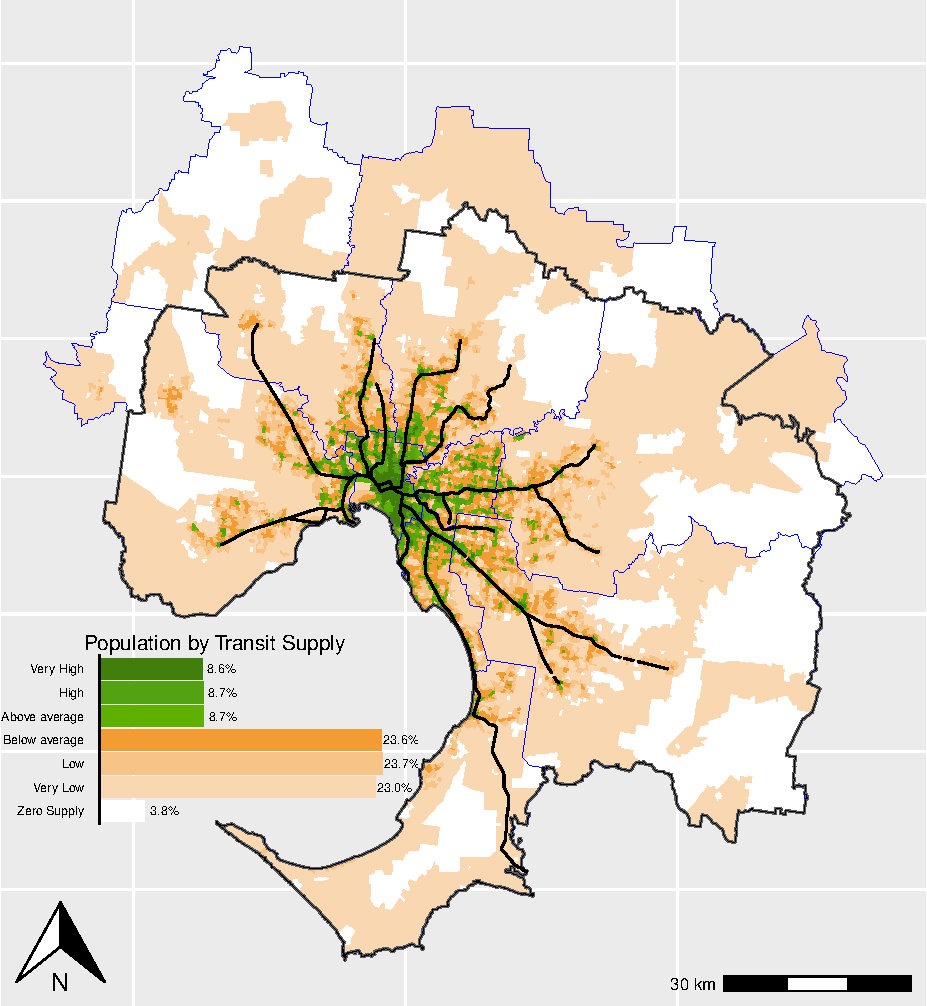
\includegraphics{ReynoldsCurrieQu2024_files/figure-latex/Greater_Melbourne_CCDs_SA1_population-1.pdf}
\caption{Greater Melbourne, Transit Supply by SA1 for the week starting
the date of the 2021 census, overlayed with: 2006 Greater Melbourne
boundary (black); 2021 SA4 boundaries (blue); and suburban railway lines
(black)}
\end{figure}

The number of people living in areas with Zero Supply rose from 85,423
(2.5\%) in 2006 to 186,829 (3.8\%) in 2021. This represents a 119\%
increase, compared to the population increase of only 46\% across all of
Greater Melbourne. The number of people with Zero or Very Low supply
rose from 878,469 (26.1\%) in 2006 to 1,319,796 (26.8\%) in 2021. This
represents a 50\% increase (4\% higher than the population change). The
number of people with a supply that was below the average (Zero, Very
Low, Low or Below Average) rose from 2,518,320 (74.8\%) in 2006 to
3,642,937 (74.1\%) in 2021. This represents a 45\% increase, which is
1\% lower than the population change.

Table \ref{tab:Greater_Melbourne_population_2016_by_SA4} and Table
\ref{tab:Greater_Melbourne_population_2021_by_SA4} show the distribution
of Transport Supply categories to the population in each SA4 zone in
2016 and 2021 respectively\^{}{[}SA4s are the largest of the statistical
boundaries used by the ABS for areas smaller than Greater Capital City
Statistical Areas (GCCSAs) or other agglomerations. The Greater
Melbourne GCCSA consists of nine SA4s, all named according to geographic
location (including the Mornington Peninsula SA4, which is at the
extreme south of the Melbourne GCCSA).

\begingroup\fontsize{8}{10}\selectfont

\begin{longtable}[t]{>{\raggedright\arraybackslash}p{1.75cm}>{\raggedleft\arraybackslash}p{1cm}>{\raggedleft\arraybackslash}p{1cm}>{\raggedleft\arraybackslash}p{1cm}>{\raggedleft\arraybackslash}p{1cm}>{\raggedleft\arraybackslash}p{1cm}>{\raggedleft\arraybackslash}p{1cm}>{\raggedleft\arraybackslash}p{1cm}>{\raggedright\arraybackslash}p{1cm}>{\raggedleft\arraybackslash}p{1cm}>{\raggedleft\arraybackslash}p{1.25cm}}
\caption{\label{tab:Greater_Melbourne_population_2016_by_SA4}Greater Melbourne 2016: Share of population in each Transport Supply category for each SA4 region}\\
\toprule
Transport Supply & Inner & Inner East & Inner South & North East & North West & Outer East & South East & West & M'ton Pen. & Total\\
\midrule
Zero Supply & 0.0\%       (0) & 0.0\%     (480) & 0.0\%   (1,604) & 0.4\%  (16,988) & 0.4\%  (17,655) & 0.3\%  (12,955) & 1.0\%  (44,757) & 0.3\%  (12,056) & 0.6\%  (25,124) & 2.9\%   (131,619)\\
Very Low & 0.1\%   (3,427) & 0.4\%  (18,454) & 0.6\%  (24,944) & 2.5\% (112,269) & 2.1\%  (94,853) & 4.3\% (190,890) & 4.8\% (215,217) & 4.2\% (186,665) & 3.6\% (161,779) & 22.5\% (1,008,498)\\
Low & 0.4\%  (18,018) & 0.9\%  (39,235) & 1.4\%  (60,833) & 2.7\% (119,608) & 2.4\% (107,693) & 3.0\% (135,247) & 5.0\% (224,097) & 5.4\% (242,438) & 1.6\%  (69,679) & 22.7\% (1,016,848)\\
Below average & 1.0\%  (42,950) & 2.3\% (105,168) & 2.9\% (128,014) & 2.9\% (132,008) & 2.2\%  (97,739) & 2.7\% (119,691) & 4.0\% (177,817) & 3.8\% (170,015) & 0.6\%  (26,888) & 22.3\% (1,000,290)\\
Above average & 1.0\%  (44,547) & 1.8\%  (80,002) & 1.8\%  (81,038) & 1.0\%  (46,965) & 0.6\%  (28,905) & 0.6\%  (25,188) & 1.2\%  (53,228) & 1.2\%  (54,895) & 0.1\%   (3,846) & 9.3\%   (418,614)\\
\addlinespace
High & 2.9\% (129,533) & 1.7\%  (74,966) & 1.7\%  (74,617) & 1.0\%  (46,291) & 0.3\%  (14,464) & 0.3\%  (15,371) & 0.7\%  (33,365) & 0.9\%  (38,499) & 0.0\%   (1,774) & 9.6\%   (428,880)\\
Very High & 7.9\% (353,232) & 0.9\%  (41,416) & 0.7\%  (32,561) & 0.5\%  (21,197) & 0.0\%   (2,033) & 0.0\%     (314) & 0.2\%   (6,893) & 0.5\%  (22,823) & 0.0\%       (0) & 10.7\%   (480,469)\\
Total & 13.2\% (591,707) & 8.0\% (359,721) & 9.0\% (403,611) & 11.0\% (495,326) & 8.1\% (363,342) & 11.1\% (499,656) & 16.8\% (755,374) & 16.2\% (727,391) & 6.4\% (289,090) & 100.0\% (4,485,218)\\
\bottomrule
\end{longtable}
\endgroup{}

\begingroup\fontsize{8}{10}\selectfont

\begin{longtable}[t]{>{\raggedright\arraybackslash}p{1.75cm}>{\raggedleft\arraybackslash}p{1cm}>{\raggedleft\arraybackslash}p{1cm}>{\raggedleft\arraybackslash}p{1cm}>{\raggedleft\arraybackslash}p{1cm}>{\raggedleft\arraybackslash}p{1cm}>{\raggedleft\arraybackslash}p{1cm}>{\raggedleft\arraybackslash}p{1cm}>{\raggedright\arraybackslash}p{1cm}>{\raggedleft\arraybackslash}p{1cm}>{\raggedleft\arraybackslash}p{1.25cm}}
\caption{\label{tab:Greater_Melbourne_population_2021_by_SA4}Greater Melbourne 2021: Share of population in each Transport Supply category for each SA4 region}\\
\toprule
Transport Supply & Inner & Inner East & Inner South & North East & North West & Outer East & South East & West & M'ton Pen. & Total\\
\midrule
Zero Supply & 0.0\%       (0) & 0.3\%     (478) & 0.9\%   (1,655) & 14.2\%  (26,563) & 11.9\%  (22,186) & 7.6\%  (14,125) & 28.9\%  (53,966) & 23.5\%  (43,898) & 12.8\%  (23,958) & 100.0\%   (186,829)\\
Very Low & 0.4\%   (4,169) & 1.8\%  (20,688) & 2.0\%  (22,483) & 11.5\% (130,715) & 9.8\% (110,814) & 17.7\% (200,810) & 22.1\% (250,684) & 19.5\% (221,337) & 15.1\% (171,267) & 100.0\% (1,132,967)\\
Low & 1.7\%  (20,329) & 3.9\%  (45,160) & 5.5\%  (63,802) & 11.3\% (132,001) & 10.6\% (123,314) & 13.4\% (155,603) & 22.9\% (265,995) & 24.9\% (289,518) & 5.8\%  (67,636) & 100.0\% (1,163,358)\\
Below average & 4.7\%  (54,918) & 11.5\% (133,305) & 12.8\% (148,585) & 13.0\% (151,240) & 11.2\% (129,918) & 9.9\% (114,658) & 17.6\% (204,093) & 15.9\% (184,466) & 3.3\%  (38,600) & 100.0\% (1,159,783)\\
Above average & 13.2\%  (56,422) & 16.2\%  (69,199) & 21.8\%  (92,875) & 10.4\%  (44,470) & 6.4\%  (27,140) & 5.2\%  (22,262) & 12.5\%  (53,328) & 13.0\%  (55,438) & 1.3\%   (5,758) & 100.0\%   (426,892)\\
\addlinespace
High & 35.6\% (151,439) & 17.3\%  (73,687) & 16.3\%  (69,281) & 10.3\%  (43,985) & 2.3\%   (9,710) & 2.6\%  (10,905) & 5.8\%  (24,707) & 9.7\%  (41,100) & 0.2\%     (965) & 100.0\%   (425,779)\\
Very High & 78.1\% (329,654) & 7.3\%  (30,949) & 5.7\%  (23,906) & 2.8\%  (11,752) & 0.3\%   (1,285) & 0.0\%       (0) & 1.7\%   (7,308) & 4.1\%  (17,171) & 0.0\%       (0) & 100.0\%   (422,025)\\
Total & 12.5\% (616,931) & 7.6\% (373,466) & 8.6\% (422,587) & 11.0\% (540,726) & 8.6\% (424,367) & 10.5\% (518,363) & 17.5\% (860,081) & 17.3\% (852,928) & 6.3\% (308,184) & 100.0\% (4,917,633)\\
\bottomrule
\end{longtable}
\endgroup{}

Variations in the share of SA1s in each Transport Supply category across
SA4 zones are statistically significant in both 2016
(\(\chi^2(48, N = 10289) = 6195.85\), \(p < .001\)) and 2021
(\(\chi^2(48, N = 11487) = 7250.39\), \(p < .001\))\footnote{Tables
  showing Transport Supply by number of SA1s for each SA4 are included
  in the Appendix.}. In general, outer areas of Greater
Melbourne\footnote{The North East, North West, Outer East, South East,
  West and Mornington Peninsula SA4 zones} appear to have larger shares
of residents living in areas with Transport Supply that is lower than
the average. In 2016, 2,714,128 residents (60.5\% of the total
population of Greater Melbourne) were both living outside of the inner
three SA4s and in SA1s with lower than average transport supply. By 2021
this had increased to 3,127,365 residents (63.6\% of the total
population).

\hypertarget{supply-index-scores}{%
\subsubsection{Supply Index scores}\label{supply-index-scores}}

\citet{currie2010identifying} reported an average SI score for CCDs in
2006 of 2,886.9 across Melbourne. In comparison, the average SI value
found here for 2021 (using CCDs and within the 2006 boundary) is 3,390.
SI scores of 10,922.7, 2,694.9 and 764.3 were reported for inner, middle
and outer suburbs, respectively, for 2006 in
\citet{currie2010identifying}. For 2021 the SI scores average 12,275.7
(+12\%) , 3,409.1 (+27\%) and 998.96 (31\%) respectively\footnote{The
  same grouping of LGAs to inner, middle and outer suburb groups as used
  in \citet{currie2010identifying} was used for this analysis, although
  here the City of Stonnington was allocated entirely to the middle
  grouping, whereas \citet{currie2010identifying} allocated part of this
  LGA to the inner group.}. However, the \citet{currie2010identifying}
results show 5,839 total CCDs within Melbourne, whereas the shape files
obtained for this analysis include 6,325 CCDs within the 2006 Melbourne
boundary. Hence, results found here might not be exactly comparable to
those in \citet{currie2010identifying} due to geographic
inconsistencies. Overall, however, results appear to be consistent with
there having been increases in SI scores across all parts of Melbourne
since 2006 and the general pattern of higher average SI scores in inner
(and then middle) than outer suburbs remaining unchanged.

It is, however, possible to directly compare SI scores 2016 and 2021,
using the SA1 2021 boundaries. Table
\ref{tab:Greater_Melbourne_2016_2021_ratio_map} shows changes in SI
score between 2016 and 2021 (column 1) by 2021 SA1s for the 2021
population, summarised for each SA4 zone (columns 2 to 10) and Greater
Melbourne as a whole (column 11). These are mapped in Figure
\ref{fig:Greater_Melbourne_2016_2021_ratio_map}.

\begingroup\fontsize{8}{10}\selectfont

\begin{longtable}[t]{>{\raggedright\arraybackslash}p{1.75cm}>{\raggedleft\arraybackslash}p{1cm}>{\raggedleft\arraybackslash}p{1cm}>{\raggedleft\arraybackslash}p{1cm}>{\raggedleft\arraybackslash}p{1cm}>{\raggedleft\arraybackslash}p{1cm}>{\raggedleft\arraybackslash}p{1cm}>{\raggedleft\arraybackslash}p{1cm}>{\raggedright\arraybackslash}p{1cm}>{\raggedleft\arraybackslash}p{1cm}>{\raggedleft\arraybackslash}p{1.25cm}}
\caption{\label{tab:Greater_Melbourne_2016_2021_ratio_map}Greater Melbourne: Share of 2021 population living in SA1s by change in transit service (2016 vs 2021) by SA4 region}\\
\toprule
Change & Inner & Inner East & Inner South & North East & North West & Outer East & South East & West & M'ton Pen. & Total\\
\midrule
New service & 0.0\%       (0) & 0.0\%       (0) & 0.0\%       (0) & 0.2\%   (9,911) & 0.7\%  (36,817) & 0.0\%     (238) & 1.1\%  (53,254) & 0.8\%  (40,483) & 0.1\%   (3,038) & 2.9\%   (143,741)\\
Increased 30\% or more & 0.0\%   (1,843) & 0.0\%     (279) & 0.8\%  (37,932) & 0.9\%  (46,448) & 1.7\%  (83,007) & 0.1\%   (4,209) & 2.6\% (127,248) & 2.7\% (131,194) & 1.3\%  (65,724) & 10.1\%   (497,884)\\
Increased 10 to 30\% & 0.9\%  (45,197) & 0.1\%   (3,190) & 0.8\%  (41,577) & 0.8\%  (40,989) & 1.1\%  (56,013) & 0.5\%  (22,609) & 1.6\%  (77,391) & 2.1\% (101,767) & 0.4\%  (21,060) & 8.3\%   (409,793)\\
Increased 5 to 10\% & 1.5\%  (72,360) & 0.3\%  (13,018) & 1.1\%  (52,033) & 0.8\%  (37,258) & 0.6\%  (31,400) & 0.5\%  (26,666) & 1.1\%  (53,370) & 2.1\% (101,769) & 0.2\%  (10,149) & 8.1\%   (398,023)\\
Increased 3 to 5\% & 1.6\%  (79,047) & 0.5\%  (25,074) & 0.6\%  (30,595) & 1.2\%  (60,661) & 1.1\%  (55,445) & 0.5\%  (23,819) & 0.9\%  (45,773) & 1.8\%  (88,601) & 0.3\%  (14,666) & 8.6\%   (423,681)\\
\addlinespace
Increased 1 to 3\% & 2.3\% (115,203) & 1.4\%  (67,357) & 1.2\%  (60,889) & 1.9\%  (92,896) & 0.9\%  (42,761) & 0.8\%  (39,263) & 1.5\%  (75,676) & 2.4\% (117,967) & 0.7\%  (32,811) & 13.1\%   (644,823)\\
Within 1\% & 2.6\% (128,666) & 3.8\% (187,974) & 2.0\%  (97,037) & 2.5\% (124,942) & 1.2\%  (57,899) & 5.6\% (274,423) & 5.4\% (266,787) & 3.0\% (146,702) & 2.2\% (109,151) & 28.3\% (1,393,581)\\
Reduced 1 to 3\% & 1.0\%  (49,729) & 0.8\%  (39,675) & 0.6\%  (27,179) & 0.7\%  (34,180) & 0.3\%  (13,986) & 0.8\%  (38,826) & 0.7\%  (34,125) & 0.4\%  (19,517) & 0.4\%  (18,446) & 5.6\%   (275,663)\\
Reduced 3 to 10\% & 1.8\%  (89,662) & 0.5\%  (25,930) & 0.9\%  (42,701) & 0.9\%  (44,261) & 0.2\%  (11,175) & 0.9\%  (43,143) & 0.5\%  (24,903) & 0.7\%  (33,329) & 0.2\%   (7,953) & 6.6\%   (323,057)\\
Reduced 10\% or more & 0.7\%  (35,224) & 0.2\%  (10,491) & 0.6\%  (30,989) & 0.5\%  (22,617) & 0.3\%  (13,678) & 0.6\%  (31,042) & 1.0\%  (47,588) & 0.6\%  (27,701) & 0.0\%   (1,228) & 4.5\%   (220,558)\\
\addlinespace
Service withdrawn (magenta) & 0.0\%       (0) & 0.0\%       (0) & 0.0\%       (0) & 0.0\%   (1,777) & 0.0\%     (424) & 0.0\%   (1,270) & 0.0\%   (1,360) & 0.0\%   (1,015) & 0.0\%       (0) & 0.1\%     (5,846)\\
Never served (black) & 0.0\%       (0) & 0.0\%     (478) & 0.0\%   (1,655) & 0.5\%  (24,786) & 0.4\%  (21,762) & 0.3\%  (12,855) & 1.1\%  (52,606) & 0.9\%  (42,883) & 0.5\%  (23,958) & 3.7\%   (180,983)\\
Total & 12.5\% (616,931) & 7.6\% (373,466) & 8.6\% (422,587) & 11.0\% (540,726) & 8.6\% (424,367) & 10.5\% (518,363) & 17.5\% (860,081) & 17.3\% (852,928) & 6.3\% (308,184) & 100.0\% (4,917,633)\\
\bottomrule
\end{longtable}
\endgroup{}

\begin{figure}
\centering
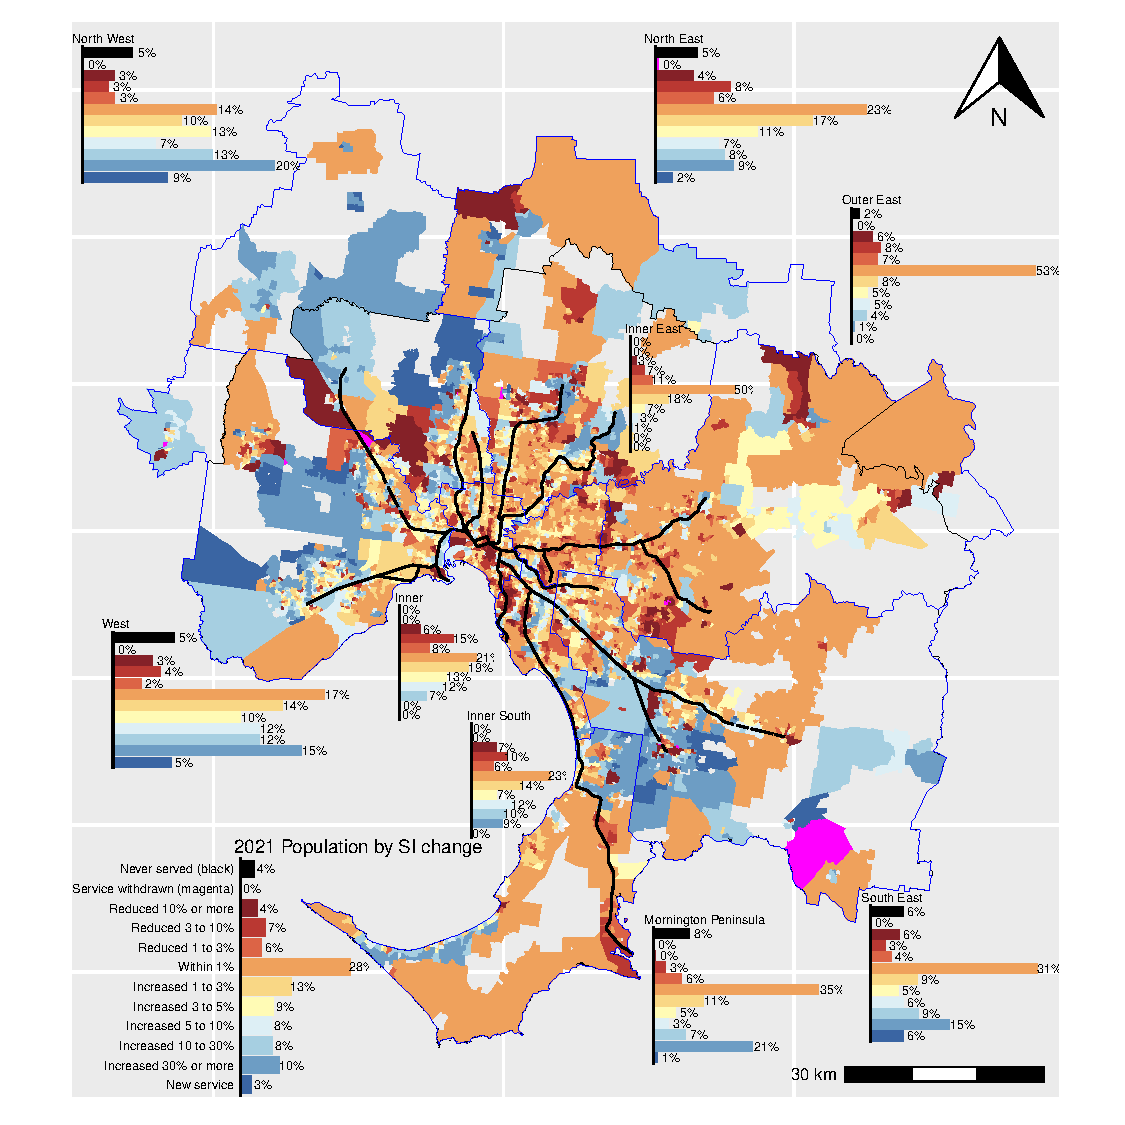
\includegraphics{ReynoldsCurrieQu2024_files/figure-latex/Greater_Melbourne_2016_2021_ratio_map-1.pdf}
\caption{Greater Melbourne: changes in SI between 2016 and 2021, by 2021
SA1, overlayed with 2006 Greater Melbourne boundary (black); 2021 SA4
boundaries (blue); and suburban railway lines (black)}
\end{figure}

Average SI scores for all of Greater Melbourne increased from 2,843.8 to
2,901.4 (+2.0\%). There is a statistically significant and strong
correlation between the 2016 and 2021 SI scores (\(r(11485) = 1.00\),
\(p < .001\), \(r_s =.98\), \(p < .001\)).

There is a statistically significant difference in the proportion of
SA1s in each service level change category across SA4 areas
(\(\chi^2(NA) = 2829.67\), \(p < .001\))\footnote{See Appendix for table}.
In 2021, more than half of the population were living in SA1s where the
SI scores were more than one percent higher than in 2016 in the
North-West (305,443 people, 72.0\%) and West (581,781 people, 68.2\%)
SA4s. This compares to slightly more than half of the population across
Greater Melbourne as a whole (2,517,945 people, 51.2\%), and less an a
third in the Inner East (108,918 people, 29.2\%) and Outer East (116,804
people, 22.5\%) SA4s.

Service levels in 2021 stayed within one percent of the level in 2016
for most of the people living in the Outer East (274,423 people, 52.9\%)
and Inner East (187,974 people, 50.3\%). For Greater Melbourne as a
whole\\
1,393,581 people ( 28.3\%) where living in SA1s in 2021 where the SI
scores had remainded within one percent of the 2016 value.

In 2021, the share of the population living in SA1s where the SI was
more than one percent lower than in 2016 was largest in the Inner
(174,615 people, 28.3\%), Inner South (100,869 people, 23.9\%) and Outer
East (114,281 people, 22.0\%) SA4s. Accross all of Greater Melbourne
825,124 people, 16.8\%) were living in SA1s in 2021 was more than one
percent lower than it had been in 2016.

In 2021 180,983 residents of Greater Melbourne ( 3.7\%) were living in
SA1s that did not have transit service in 2016 or 2021. The largest
proportions were amongst the Mornington Peninsula (7.8\%, 23,958) and
South East (6.1\%, 52,606) SA4s, whereas no one at all in the Inner SA4
was living in a SA1 without at least a Very Low service level.

\hypertarget{social-needs}{%
\subsubsection{Social needs}\label{social-needs}}

\begin{figure}
\centering
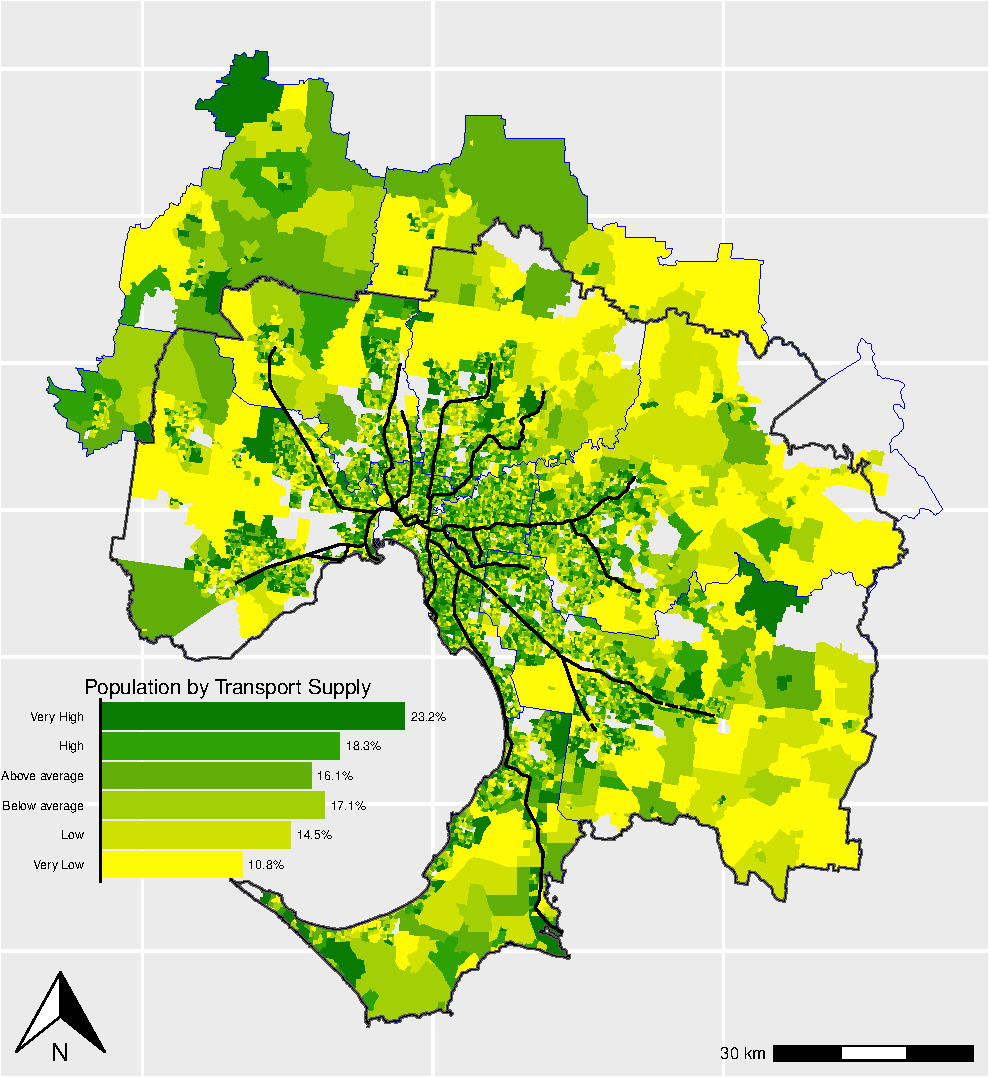
\includegraphics{ReynoldsCurrieQu2024_files/figure-latex/Greater_Melbourne_2021_social_needs-1.pdf}
\caption{Distribution of categories of composite social need index
scores, overlayed with: 2006 Greater Melbourne boundary (black); SA4
boundaries (blue); and suburban railway lines (dashed).}
\end{figure}

Figure \ref{fig:Greater_Melbourne_2021_social_needs} shows the
distribution of categories of social need index scores across Greater
Melbourne for 2021\footnote{A map for 2016 is included in the Appendix
  as Figure \ref{fig:Greater_Melbourne_2016_social_needs_appendix}}.
This is analogous to the 2006 map shown in Figure
\ref{fig:Currie_map_SI} (b) although, as discussed in the methodology
section above, it was not possible to exactly replicate the
\citet{currie2010identifying} social needs scoring approach due to
changes in the way census results are reported. In general, the spatial
grouping of different levels of social need appears less consistently
grouped in 2021 than in 2006, although this may be an artifact of the
shift to SA1s from CCDs\footnote{CCDs were originally devised to group
  the approximately 200 dwellings allocated to each individual census
  collector, whereas SA1s were introduced to be consistent in population
  (200 to 800 people, averaging 400) and character \citep{ABS_SA1s_CCDs}}.

\hypertarget{needs-gap}{%
\subsubsection{Needs-gap}\label{needs-gap}}

\begin{figure}
\centering
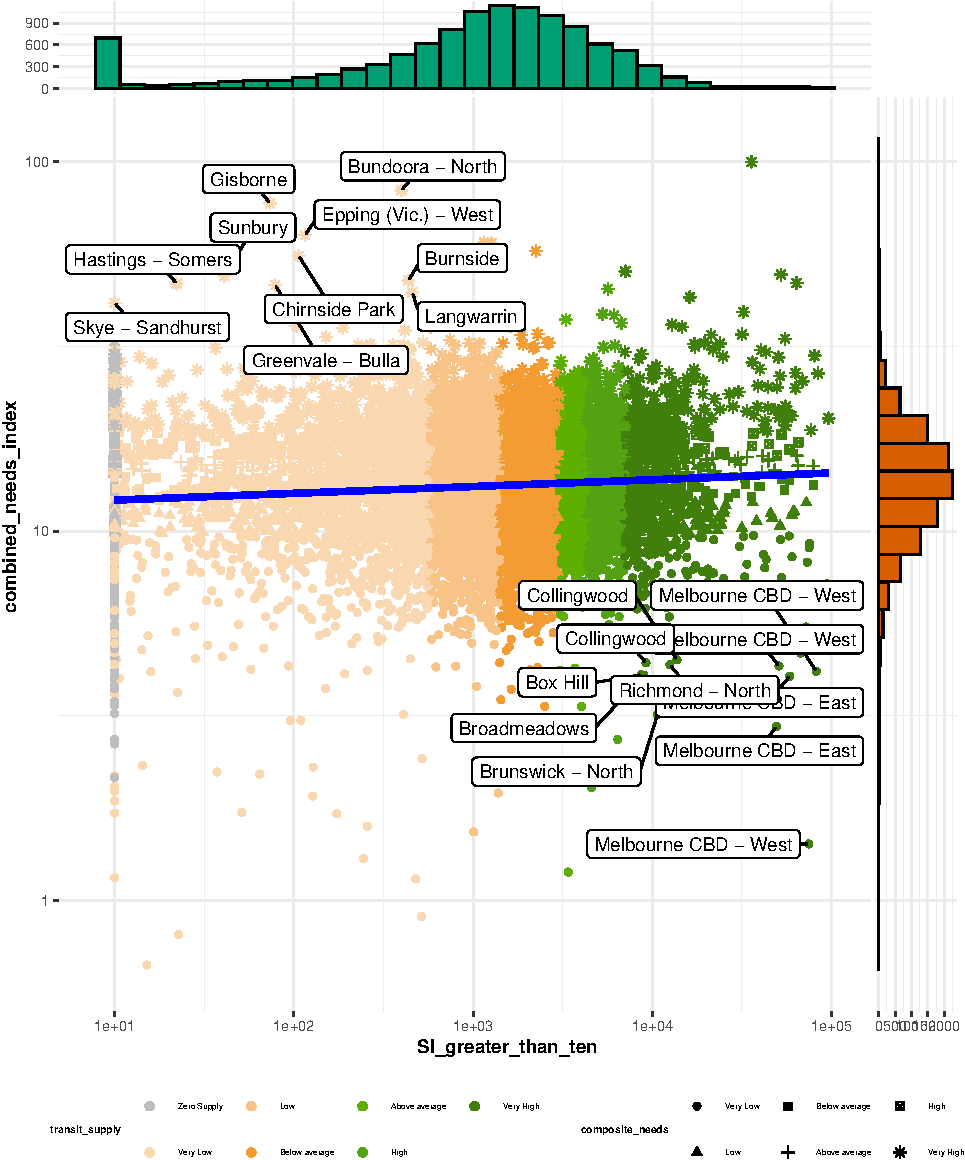
\includegraphics{ReynoldsCurrieQu2024_files/figure-latex/Greater_Melbourne_2021_needs_gap_scatterplot_figure-1.pdf}
\caption{Greater Melbourne 2021, SI and Combined Needs Index scores,
with SI scores \textless{} 10 rounded up to equal 10 to improve
clarity.}
\end{figure}

Figures \ref{fig:Greater_Melbourne_2016_needs_gap_scatterplot_figure}
and \ref{fig:Greater_Melbourne_2016_needs_gap_scatterplot_figure} show
social needs and SI scores\footnote{To improve the clarity of the
  figure, SI scores less than 10 have been adjusted to equal 10.}. Those
SA1s with combinations of Zero or Very Low transit supply and
(especially) high needs scores (more than 40); or Very High supply and
Very Low needs scores (less than 4.5) have been labelled with their SA2
name, so as to given an indication of which suburbs of Melbourne are at
each of the extremes. There is a significant, but only weakly positive
correlation between the SI and Combined Needs Index scores for both 2016
(\(r(11136) = .06\), \(p < .001\), \(r_s =.07\), \(p < .001\)) and 2021
(\(r(11136) = .06\), \(p < .001\), \(r_s =.07\), \(p < .001\)).

Table \ref{tab:Greater_Melbourne_2016_needs_gap_population} compares the
populations within each Transport Supply and Combined Needs Index
grouping for 2016. There is a statistically significant relationship
(\(\chi^2(30, N = 4471171) = 158778.27\), \(p < .001\)). 301,743 people
live within SA1s that have Zero or Very Low transport supply, but Very
High social needs. This represents 6.7\% of the 4,471,171 people within
Greater Melbourne, and is higher proportion than that reported for 2006
(139,004 of 3.3 million people (4.2\%)). These areas are mapped for by
2016 and 2021 in Figure
\ref{fig:Greater_Melbourne_2016_needs_gap_map_figure}

Table \ref{tab:Greater_Melbourne_2021_needs_gap_population} shows the
same comparison for 2021. There is a statistically significant
relationship (\(\chi^2(30, N = 4904313) = 55715.62\), \(p < .001\)).
333,887 people live within SA1s that have Zero or Very Low transport
supply, but Very High social needs. This represents 6.8\% of the
4,904,313 people within Greater Melbourne, which is higher than that
reported for both 2006 and 2016.

\begingroup\fontsize{8}{10}\selectfont

\begin{longtable}[t]{>{\raggedright\arraybackslash}p{2.5cm}>{\raggedleft\arraybackslash}p{1cm}>{\raggedleft\arraybackslash}p{1cm}>{\raggedleft\arraybackslash}p{1cm}>{\raggedright\arraybackslash}p{1cm}>{\raggedleft\arraybackslash}p{1cm}>{\raggedleft\arraybackslash}p{1cm}>{\raggedleft\arraybackslash}p{1.5cm}}
\caption{\label{tab:Greater_Melbourne_2016_needs_gap_population}Greater Melbourne 2016, Population in each SI and Combined Needs Index grouping}\\
\toprule
\multicolumn{1}{c}{ } & \multicolumn{6}{c}{Combined Needs Index Category} & \multicolumn{1}{c}{ } \\
\cmidrule(l{3pt}r{3pt}){2-7}
Supply & Very High & High & Above Average & Below Average & Low & Very Low & Total\\
\midrule
Zero Supply & 0.9\%    (38,050) & 0.3\%  (14,790) & 0.3\%  (15,402) & 0.4\%  (18,784) & 0.5\%  (22,544) & 0.5\%  (22,012) & 2.9\%   (131,582)\\
Very Low & 5.9\%   (263,693) & 3.4\% (153,169) & 3.1\% (138,710) & 3.7\% (165,350) & 3.5\% (156,359) & 2.8\% (126,298) & 22.4\% (1,003,579)\\
Low & 4.5\%   (200,937) & 3.8\% (168,541) & 3.5\% (154,275) & 4.4\% (197,542) & 3.8\% (168,228) & 2.8\% (126,411) & 22.7\% (1,015,934)\\
Below average & 3.7\%   (164,681) & 4.0\% (177,044) & 3.7\% (163,593) & 4.3\% (193,915) & 3.8\% (169,849) & 2.9\% (129,440) & 22.3\%   (998,522)\\
Above average & 1.9\%    (84,562) & 1.8\%  (80,172) & 1.6\%  (70,066) & 1.8\%  (80,591) & 1.4\%  (61,679) & 0.8\%  (38,003) & 9.3\%   (415,073)\\
\addlinespace
High & 2.4\%   (105,960) & 2.0\%  (89,517) & 1.5\%  (67,061) & 1.9\%  (83,055) & 1.1\%  (49,615) & 0.7\%  (33,334) & 9.6\%   (428,542)\\
Very High & 4.3\%   (192,038) & 1.8\%  (79,329) & 1.5\%  (68,467) & 1.3\%  (56,303) & 1.1\%  (48,441) & 0.7\%  (33,361) & 10.7\%   (477,939)\\
Total & 23.5\% (1,049,921) & 17.1\% (762,562) & 15.2\% (677,574) & 17.8\% (795,540) & 15.1\% (676,715) & 11.4\% (508,859) & 100.0\% (4,471,171)\\
\bottomrule
\end{longtable}
\endgroup{}

\begingroup\fontsize{8}{10}\selectfont

\begin{longtable}[t]{>{\raggedright\arraybackslash}p{2.5cm}>{\raggedleft\arraybackslash}p{1cm}>{\raggedleft\arraybackslash}p{1cm}>{\raggedleft\arraybackslash}p{1cm}>{\raggedright\arraybackslash}p{1cm}>{\raggedleft\arraybackslash}p{1cm}>{\raggedleft\arraybackslash}p{1cm}>{\raggedleft\arraybackslash}p{1.5cm}}
\caption{\label{tab:Greater_Melbourne_2021_needs_gap_population}Greater Melbourne 2021, Population in each SI and Combined Needs Index grouping}\\
\toprule
\multicolumn{1}{c}{ } & \multicolumn{6}{c}{Combined Needs Index Category} & \multicolumn{1}{c}{ } \\
\cmidrule(l{3pt}r{3pt}){2-7}
Supply & Very High & High & Above Average & Below Average & Low & Very Low & Total\\
\midrule
Zero Supply & 0.9\%    (41,915) & 0.6\%  (27,179) & 0.5\%  (22,705) & 0.7\%  (32,328) & 0.7\%  (32,645) & 0.6\%  (30,002) & 3.8\%   (186,774)\\
Very Low & 6.0\%   (291,972) & 4.1\% (199,467) & 3.4\% (165,968) & 3.7\% (182,624) & 3.2\% (158,222) & 2.6\% (129,608) & 23.0\% (1,127,861)\\
Low & 4.9\%   (239,199) & 4.2\% (205,465) & 3.9\% (193,243) & 4.3\% (210,576) & 3.7\% (183,333) & 2.7\% (130,779) & 23.7\% (1,162,595)\\
Below average & 4.7\%   (228,646) & 4.5\% (219,310) & 4.2\% (204,049) & 4.2\% (203,750) & 3.5\% (171,997) & 2.7\% (130,322) & 23.6\% (1,158,074)\\
Above average & 2.0\%   (100,326) & 1.6\%  (80,404) & 1.5\%  (73,669) & 1.6\%  (76,179) & 1.2\%  (56,902) & 0.8\%  (37,419) & 8.7\%   (424,899)\\
\addlinespace
High & 2.2\%   (107,121) & 1.7\%  (83,970) & 1.4\%  (70,132) & 1.6\%  (77,358) & 1.1\%  (54,528) & 0.7\%  (32,274) & 8.7\%   (425,383)\\
Very High & 2.6\%   (129,759) & 1.6\%  (79,306) & 1.2\%  (59,356) & 1.1\%  (55,828) & 1.1\%  (54,061) & 0.8\%  (40,417) & 8.5\%   (418,727)\\
Total & 23.2\% (1,138,938) & 18.3\% (895,101) & 16.1\% (789,122) & 17.1\% (838,643) & 14.5\% (711,688) & 10.8\% (530,821) & 100.0\% (4,904,313)\\
\bottomrule
\end{longtable}
\endgroup{}

\begin{figure}

{\centering \subfloat[2016\label{fig:Greater_Melbourne_2016_needs_gap_map_figure-1}]{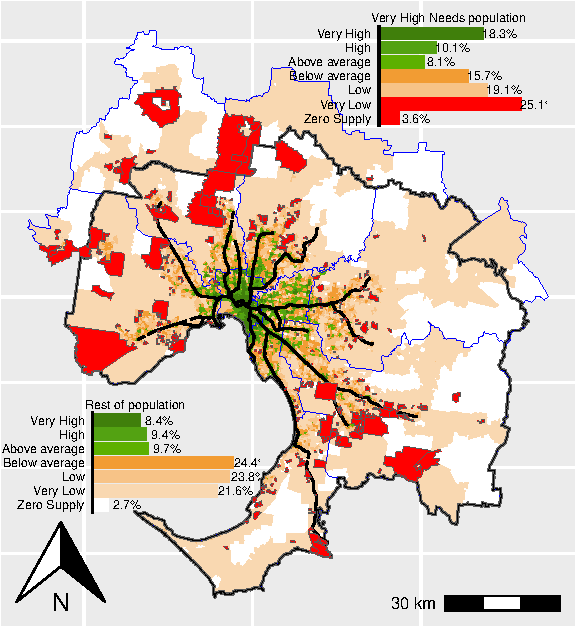
\includegraphics[width=0.5\linewidth]{ReynoldsCurrieQu2024_files/figure-latex/Greater_Melbourne_2016_needs_gap_map_figure-1} }\subfloat[2021\label{fig:Greater_Melbourne_2016_needs_gap_map_figure-2}]{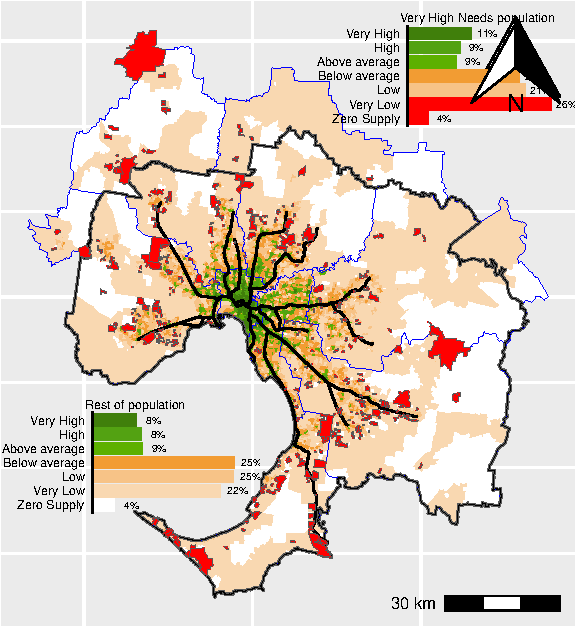
\includegraphics[width=0.5\linewidth]{ReynoldsCurrieQu2024_files/figure-latex/Greater_Melbourne_2016_needs_gap_map_figure-2} }

}

\caption{Greater Melbourne Transport Supply groupings overlayed with SA1s with very high transport need areas with zero or very low public transport supply (red).}\label{fig:Greater_Melbourne_2016_needs_gap_map_figure}
\end{figure}

Figures \ref{fig:Greater_Melbourne_2016_needs_gap_map_figure} and
\ref{fig:Greater_Melbourne_2021_needs_gap_map_figure} show SA1 zones in
Greater Melbourne with Very High transport needs, but Very Low or Zero
transit supply for 2016 and 2021. Comparison to the 2006 spatial
distribution shown in Figure \ref{fig:Currie_map_SI} (bottom) suggests
that areas with large gaps between social needs and transit supply
continue to be mostly in the outer areas of Melbourne. However, such
comparisons appear complicated by the larger number of SA1s than CCDs,
with Figures \ref{fig:Greater_Melbourne_2016_needs_gap_map_figure} and
\ref{fig:Greater_Melbourne_2021_needs_gap_map_figure} appearing to show
more (smaller) areas with Very High transport needs, but Very Low or
Zero transit supply. This includes areas in the West, North West, North
East and South East SA4s, whereas in 2006 these parts of Melbourne did
not appear to have large gaps between need and supply. The bottom parts
of the Morning Peninsula (around Blairgowrie) drop out of the category
of having the largest needs-gaps in 2016, but are back in this category
again in 2021.

\hypertarget{needs-gap-and-service-level-changes}{%
\subsubsection{Needs-gap and service level
changes}\label{needs-gap-and-service-level-changes}}

Tables \ref{Greater_Melbourne_2016_needs_gap_SA4_service_change} and
\ref{Greater_Melbourne_2021_needs_gap_SA4_service_change} show how
service levels changed for those SA1 areas that had Very High needs but
Very Low or Zero service. These are summarised across S4 areas by
population for 2016 and 2021.

\begingroup\fontsize{8}{10}\selectfont

\begin{longtable}[t]{>{\raggedright\arraybackslash}p{1.75cm}>{\raggedleft\arraybackslash}p{1cm}>{\raggedleft\arraybackslash}p{1cm}>{\raggedleft\arraybackslash}p{1cm}>{\raggedleft\arraybackslash}p{1cm}>{\raggedleft\arraybackslash}p{1cm}>{\raggedleft\arraybackslash}p{1cm}>{\raggedleft\arraybackslash}p{1cm}>{\raggedright\arraybackslash}p{1cm}>{\raggedleft\arraybackslash}p{1.25cm}}
\caption{\label{tab:Greater_Melbourne_2016_needs_gap_SA4_service_change}Greater Melbourne: 2016 residents living in areas with Very High needs but Very Low or Zero supply, by SA4 and change in SI by 2021}\\
\toprule
Change & Inner & Inner South & North East & North West & Outer East & South East & West & M'ton Pen. & Total\\
\midrule
New service & 0.0\%     (0) & 0.0\%     (0) & 0.7\%  (1,877) & 0.8\%  (2,335) & 0.0\%      (0) & 5.8\% (16,769) & 0.5\%  (1,461) & 0.2\%    (702) & 8.1\%  (23,144)\\
Increased 30\% or more & 0.0\%     (0) & 0.5\% (1,512) & 3.2\%  (9,051) & 6.8\% (19,372) & 0.0\%      (0) & 9.9\% (28,348) & 10.8\% (31,091) & 1.6\%  (4,640) & 32.8\%  (94,014)\\
Increased 10 to 30\% & 0.0\%     (0) & 0.0\%     (0) & 2.0\%  (5,833) & 2.6\%  (7,576) & 0.9\%  (2,528) & 2.9\%  (8,253) & 1.8\%  (5,067) & 0.0\%      (0) & 10.2\%  (29,257)\\
Increased 5 to 10\% & 0.0\%     (0) & 0.0\%     (0) & 0.7\%  (2,067) & 0.0\%      (0) & 0.5\%  (1,452) & 2.1\%  (6,119) & 2.8\%  (8,145) & 0.3\%    (791) & 6.5\%  (18,574)\\
Increased 3 to 5\% & 0.0\%     (0) & 0.0\%     (0) & 0.2\%    (566) & 0.5\%  (1,397) & 0.2\%    (603) & 1.3\%  (3,586) & 0.8\%  (2,378) & 0.9\%  (2,487) & 3.8\%  (11,017)\\
\addlinespace
Increased 1 to 3\% & 0.2\%   (568) & 0.2\%   (648) & 0.6\%  (1,706) & 0.0\%      (0) & 0.4\%  (1,260) & 0.5\%  (1,575) & 2.5\%  (7,233) & 1.0\%  (2,910) & 5.5\%  (15,900)\\
Within 1\% & 0.2\%   (546) & 0.4\% (1,271) & 2.0\%  (5,639) & 0.3\%    (953) & 5.1\% (14,489) & 5.6\% (15,974) & 4.3\% (12,378) & 4.3\% (12,421) & 22.2\%  (63,671)\\
Reduced 1 to 3\% & 0.0\%     (0) & 0.2\%   (585) & 0.4\%  (1,249) & 0.0\%      (0) & 0.2\%    (600) & 0.0\%      (0) & 0.7\%  (2,009) & 0.8\%  (2,349) & 2.4\%   (6,792)\\
Reduced 3 to 10\% & 0.0\%     (0) & 0.2\%   (557) & 3.0\%  (8,695) & 0.0\%      (0) & 0.2\%    (612) & 0.7\%  (1,910) & 1.9\%  (5,550) & 0.6\%  (1,648) & 6.6\%  (18,972)\\
Reduced 10\% or more & 0.0\%     (0) & 0.2\%   (611) & 0.3\%    (825) & 0.2\%    (670) & 0.4\%  (1,192) & 0.5\%  (1,535) & 0.0\%      (0) & 0.0\%      (0) & 1.7\%   (4,833)\\
\addlinespace
Service withdrawn (magenta) & 0.0\%     (0) & 0.0\%     (0) & 0.0\%      (0) & 0.0\%      (0) & 0.2\%    (663) & 0.0\%      (0) & 0.0\%      (0) & 0.0\%      (0) & 0.2\%     (663)\\
Total & 0.4\% (1,114) & 1.8\% (5,184) & 13.1\% (37,508) & 11.3\% (32,303) & 8.2\% (23,399) & 29.3\% (84,069) & 26.3\% (75,312) & 9.7\% (27,948) & 100.0\% (286,837)\\
\bottomrule
\end{longtable}
\endgroup{}

\begingroup\fontsize{8}{10}\selectfont

\begin{longtable}[t]{>{\raggedright\arraybackslash}p{1.75cm}>{\raggedleft\arraybackslash}p{1cm}>{\raggedleft\arraybackslash}p{1cm}>{\raggedleft\arraybackslash}p{1cm}>{\raggedleft\arraybackslash}p{1cm}>{\raggedleft\arraybackslash}p{1cm}>{\raggedleft\arraybackslash}p{1cm}>{\raggedleft\arraybackslash}p{1cm}>{\raggedright\arraybackslash}p{1cm}>{\raggedleft\arraybackslash}p{1.25cm}}
\caption{\label{tab:Greater_Melbourne_2021_needs_gap_SA4_service_change}Greater Melbourne: 2021 residents living in areas with Very High needs but Very Low or Zero supply, by SA4 and change in SI since 2016}\\
\toprule
Change & Inner & Inner South & North East & North West & Outer East & South East & West & M'ton Pen. & Total\\
\midrule
New service & 0.0\%     (0) & 0.0\%     (0) & 1.0\%  (3,306) & 2.1\%  (6,767) & 0.0\%      (0) & 5.7\% (18,099) & 3.3\% (10,411) & 0.4\%  (1,404) & 12.5\%  (39,987)\\
Increased 30\% or more & 0.0\%     (0) & 0.0\%     (0) & 2.5\%  (8,091) & 4.4\% (13,910) & 0.0\%      (0) & 4.5\% (14,299) & 4.4\% (13,985) & 2.1\%  (6,662) & 17.8\%  (56,947)\\
Increased 10 to 30\% & 0.0\%     (0) & 0.0\%     (0) & 1.2\%  (3,917) & 2.3\%  (7,264) & 0.8\%  (2,692) & 2.0\%  (6,416) & 1.3\%  (4,127) & 0.2\%    (500) & 7.8\%  (24,916)\\
Increased 5 to 10\% & 0.0\%     (0) & 0.0\%     (0) & 0.6\%  (1,869) & 0.0\%      (0) & 0.5\%  (1,457) & 1.4\%  (4,328) & 2.3\%  (7,305) & 0.4\%  (1,434) & 5.1\%  (16,393)\\
Increased 3 to 5\% & 0.0\%     (0) & 0.0\%     (0) & 0.2\%    (550) & 0.9\%  (2,835) & 0.2\%    (613) & 0.6\%  (1,919) & 0.7\%  (2,194) & 0.8\%  (2,600) & 3.4\%  (10,711)\\
\addlinespace
Increased 1 to 3\% & 0.2\%   (587) & 0.2\%   (727) & 0.8\%  (2,597) & 0.0\%      (0) & 0.2\%    (712) & 0.6\%  (1,873) & 2.3\%  (7,442) & 1.2\%  (3,706) & 5.5\%  (17,644)\\
Within 1\% & 0.2\%   (571) & 0.6\% (1,986) & 1.8\%  (5,696) & 0.9\%  (3,011) & 5.5\% (17,628) & 6.6\% (21,156) & 5.0\% (15,915) & 5.1\% (16,381) & 25.8\%  (82,344)\\
Reduced 1 to 3\% & 0.0\%     (0) & 0.2\%   (581) & 0.4\%  (1,341) & 0.2\%    (726) & 0.2\%    (618) & 0.2\%    (577) & 0.8\%  (2,416) & 1.0\%  (3,250) & 3.0\%   (9,509)\\
Reduced 3 to 10\% & 0.0\%     (0) & 0.2\%   (583) & 1.5\%  (4,926) & 0.4\%  (1,247) & 0.8\%  (2,413) & 0.4\%  (1,349) & 1.4\%  (4,341) & 1.3\%  (4,169) & 6.0\%  (19,028)\\
Service withdrawn (magenta) & 0.0\%     (0) & 0.0\%     (0) & 0.4\%  (1,315) & 0.0\%      (0) & 0.2\%    (630) & 0.2\%    (718) & 0.0\%      (0) & 0.0\%      (0) & 0.8\%   (2,663)\\
\addlinespace
Never served (black) & 0.0\%     (0) & 0.2\%   (725) & 1.5\%  (4,900) & 1.4\%  (4,481) & 0.0\%      (0) & 4.0\% (12,847) & 4.0\% (12,742) & 1.1\%  (3,557) & 12.3\%  (39,252)\\
Total & 0.4\% (1,158) & 1.4\% (4,602) & 12.1\% (38,508) & 12.6\% (40,241) & 8.4\% (26,763) & 26.2\% (83,581) & 25.3\% (80,878) & 13.7\% (43,663) & 100.0\% (319,394)\\
\bottomrule
\end{longtable}
\endgroup{}

There is a significant difference across SA4s in 2016
(\(\chi^2(NA) = 148541.79\), \(p < .001\)) and 2021
(\(\chi^2(NA) = 109675.47\), \(p < .001\)). Of those people living in
SA1s that Very High needs but Very Low or Zero service in 2016, those
living in the North West, South East and West were more likely to have
received some new or additional transit service by 2021. For those
living in the Outer East, Inner South and Mornington Peninsula service
levels were more likely to have stayed within one percent or been
reduced, or (for 663 people living in the Outer East (2.8\%)) had their
Service withdrawn (magenta) entirely.

A larger proportion of those living in the Inner South, North East, West
or Mornington Peninsula who were living in SA1s with Very High needs but
Very Low or Zero service in 2021 had seen service levels reduced by more
than one percent or had services withdrawn entirely or not providing in
2016 or 2021. This included the 4,900 people living in the North East
(12.7\% of residents) and 12,847 people living in the South East (15.4\%
of residents). A further 0 people living in the Outer East in 2021
(0.0\% of residents) were living in SA1s with Very High needs but Very
Low or Zero service in 2021, which had some transit service in 2016 but
none in 2021. A larger proportion of the population were living in SA1s
with Very High needs but Very Low or Zero service in 2021 had not had
service in 2016 or 2021 in the South East (NA, NA), West (NA, NA
residents), North East (NA, NA residents) and Inner South (NA, NA
residents)

Service levels had increased (by more than one percent) for those living
in SA1s with Very High needs but Very Low or Zero service in 2021 for a
larger proportion of those living in the North West (76.5\%, 30,776
residents), the South East (56.2\%, 46,934 residents) and West (56.2\%,
45,464 residents). However, even those service levels had increased,
they still remained in the Very Low category.

\hypertarget{discussion}{%
\section{Discussion}\label{discussion}}

This research was motivated by a lack of software tools to analyse gaps
between social needs for transport and the amount of transit provided,
and to better understand how spatial patterns might have changed since
the original development of this methodology in the early 2000s. The
needs-gaps approach was suggested to be ``substantially more useful than
the presentation of anecdotal evidence, which is the most common means
of identifying transport needs in local transport studies throughout the
world'' \citep{currie2010identifying}, yet this technique does not
appear to have been adopted in practice. The research reported in this
paper, therefore, is important because it may help bridge gaps between
research (where the needs-gap approach and SI formulation was developed)
and the real world of transport planning, advocacy, professional
practice and politics (where decisions are made about where transit
services are needed or need improving).

As discussed in Section 2, there are many transit metrics available, but
these may be challenging to apply or calculate independently. The SI has
the advantage of combining accessibility and service frequency into a
single measure, which is relatively simple to understand and can even be
calculated by hand for smaller networks. With the gtfstools R package
developed in this research applying the SI calculation across even
relatively large transit networks, such as that of Greater Melbourne,
requires only a GTFS feed, some computer time and a bit of data
scientist know-how (or a willingness and time to learn). The tool is not
yet at a download, point and click level of useability. However, it is
open source and publicly available, and so may make it easier to assess
transit service levels and network change proposals with respect to
social needs for transport.

The maps, graphs, tables and other outputs presented in this paper also
demonstrate the range of analysis that might be possible using this
package. Longitudinal comparison of transit service levels has been
shown in aggregate (Table
\ref{tab:Greater_Melbourne_CCDs_SA1_population}), by population across
sub-areas (in comparing Tables
\ref{tab:Greater_Melbourne_population_2016_by_SA4} and
\ref{tab:Greater_Melbourne_population_2016_by_SA4}) and mapped (Figure
\ref{fig:Greater_Melbourne_2016_2021_ratio_map}). Visual display of gaps
between social needs and transit supply how also been shown through
scatterplots (Figures
\ref{fig:Greater_Melbourne_2016_needs_gap_scatterplot} and
\ref{fig:Greater_Melbourne_2021_needs_gap_scatterplot}) and mapping
(Figures \ref{fig:Greater_Melbourne_2016_needs_gap_map} and
\ref{fig:Greater_Melbourne_2021_needs_gap_map}). Such outputs,
especially if produced at the spatial level of a neighbourhood, council
ward or electoral division, might provide an opportunity for advocates
and professionals within transport planning to identify and easily
demonstrate to the public, politician and other stakeholders which
spatial areas might benefit from increasing transit funding and where
funds might best be directed.

Previous research looking at bus services in new developments includes
the \citet{delbosc2015impact} case study of the Selandra Rise planned
estate in the south-east of Melbourne. This study explored the impact of
the, then newly introduced, 798 bus route (Figure \ref{fig:Bus_798}. The
route was reported as having around 2,500 boardings per week and being
used by at least one person in 35 percent of households within the
Selandra Rise Estate, despite it not penetrating fully into the
development and only 20 percent of the estate's footprint being within
400 metres of the route. Findings suggested that: the route was
``performing an important `social transit' function''; that ``those who
do use the bus use it very frequently (88 percent (of riders) at least a
few days a week)''; ``Most bus riders were young and could not drive or
had no car available, making them quite reliant on the bus'', and that
it ``frees up the time of other household members who would have had to
provide lifts'' \citep[p.10]{delbosc2015impact}. Figure
\ref{fig:Selandra_rise} revisits the Selandra Rise Estate, showing
transport supply in 2016 and 2021, and changes in SI score for SA1s with
Very High social needs, but Very Low or Zero transit supply.

\begin{figure}

{\centering 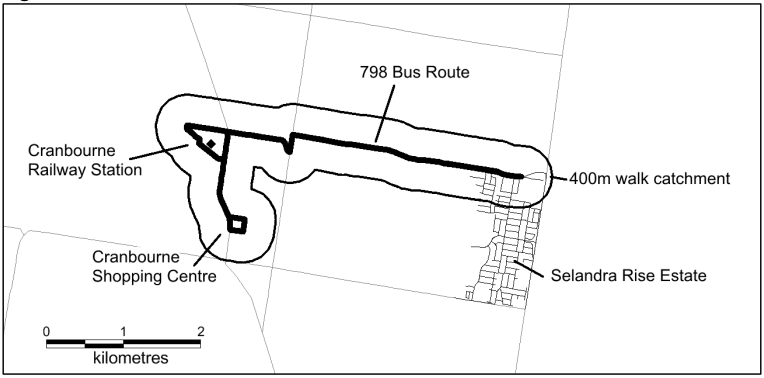
\includegraphics[width=1\linewidth]{graphics/Route798} 

}

\caption{Bus Route 798 as originally introduced in 2014 (Source: Delbosc et al (2015))}\label{fig:Bus_798}
\end{figure}

\begin{figure}

{\centering \subfloat[Transport Supply categories in 2016\label{fig:Selandra_rise-1}]{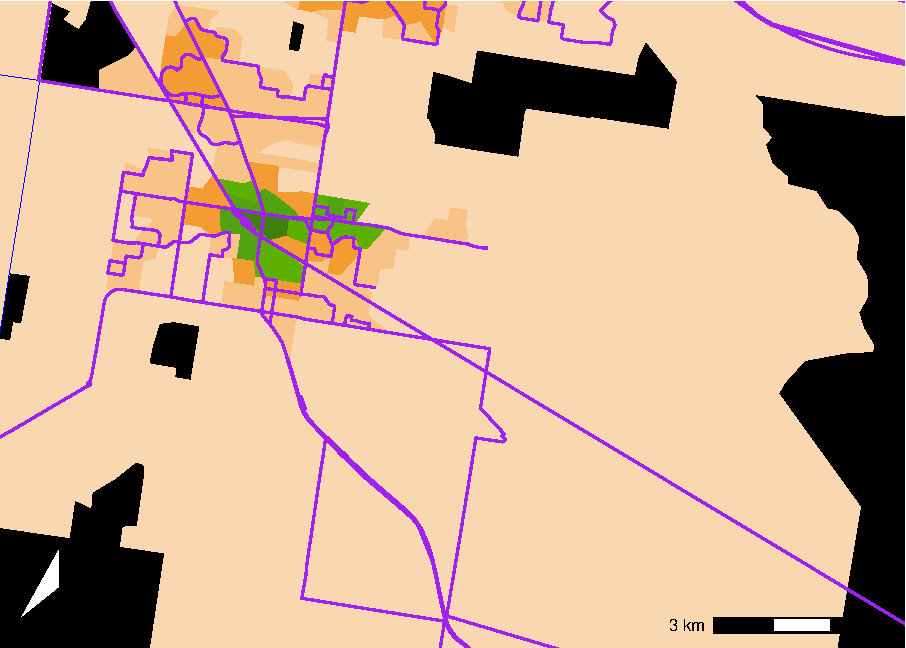
\includegraphics[width=0.5\linewidth]{ReynoldsCurrieQu2024_files/figure-latex/Selandra_rise-1} }\subfloat[Transport Supply categories in 2021 (transit routes in purple)\label{fig:Selandra_rise-2}]{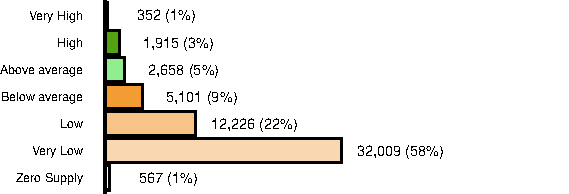
\includegraphics[width=0.5\linewidth]{ReynoldsCurrieQu2024_files/figure-latex/Selandra_rise-2} }\newline\subfloat[Change in SI score between 2016 and 2021 for SA1s with Very High needs but Very Low or Zero supply with 2021 populations\label{fig:Selandra_rise-3}]{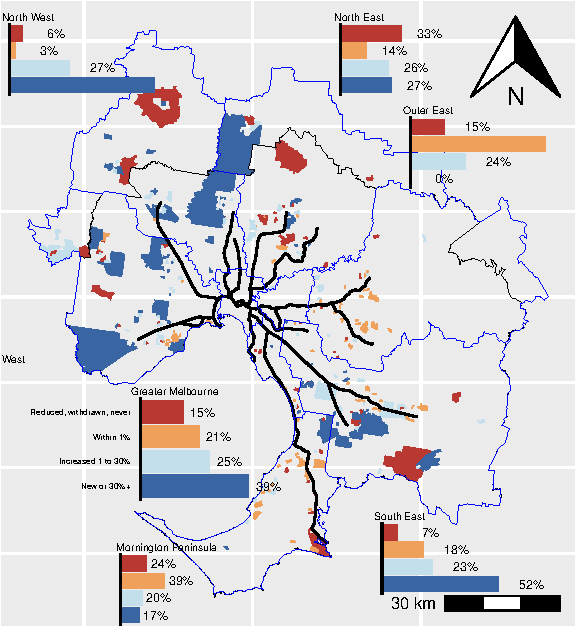
\includegraphics[width=0.5\linewidth]{ReynoldsCurrieQu2024_files/figure-latex/Selandra_rise-3} }\subfloat[Current (2024) route map\label{fig:Selandra_rise-4}]{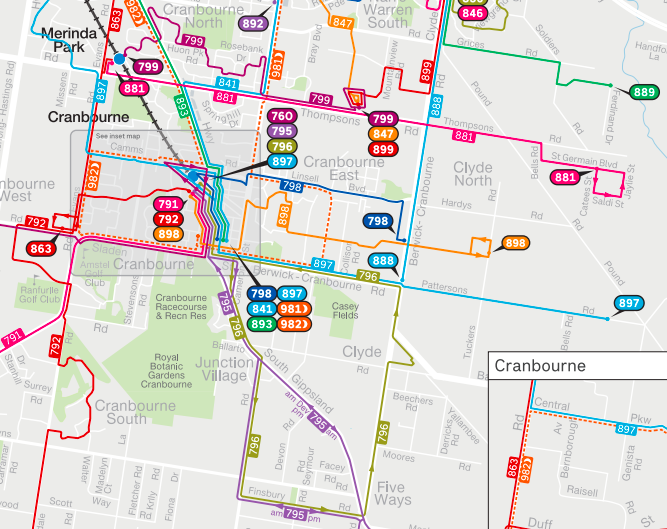
\includegraphics[width=0.5\linewidth]{graphics/Cranbourne} }\newline

}

\caption{Cranbourne and the Selandra Rise Estate (colours as per previous figures, transit routes in purple, 2016 and 2021 SA1 boundaries in grey.)}\label{fig:Selandra_rise}
\end{figure}

Various transit routes appear to have been added to the area surrounding
the Selandra Rise Estate between 2016 (Figure \ref{fig:Selandra_rise},
top-left), 2021 (top-right) and 2024 (bottom-right). After 2016 Route
798 was adjusted to penetrate into the estate, and Route 888 was added
to provide a north-south connection along Berwick-Cranbourne Road. This
appears to have been sufficient to shift some of the estate into the Low
transport supply category in 2021, up from Very Low category in 2016.
Figure \ref{fig:Selandra_rise}, bottom-left, however, indicates that
some of the surrounding SA1s, however, still fall into the Very High
needs and Very Low or Zero supply social needs-gap category, including
some SA1s that have over 700 residents but did not have a transit
service within 400 metres in either 2016 and 2021. That said, it appears
that Route 898 has been added between 2021 and 2024, providing an
additional east-west connection and coverage, suggesting that the
ultimate transit network for the area is not yet implemented.

What the information shown in the bottom-left and bottom-right of Figure
\ref{fig:Selandra_rise} might suggest, however, is that areas in the
vicinity of Casey Fields are underserved. Revising Route 795 so as to
service areas north of Ballarto Rd, perhaps instead of duplicating parts
of Route 796, might be one option to increase coverage and provide some
stops for residents living in areas that did not have an transit within
400 metres in either 2016 or 2021.

\hypertarget{conclusions}{%
\section{Conclusions}\label{conclusions}}

This paper has reported the development of a new R package containing
tools for identifying gaps between the social need for transport and the
service provided based on GTFS data. It has also demonstrated how this
package might be applied to the case of Greater Melbourne in 2016 and
2021, in the same manner in which \citet{currie2010identifying} applied
the analysis approach to Melbourne in 2006.

A motivation for this study was explore how spatial patterns related to
transport supply, need and gaps have changed in Melbourne since 2006. To
some extent the results indicate the challenges of making longitudinal
comparisons when there are changes in statistical geography. The shift
from CCDs to SA1s by the ABS appears to have allowed results to be
output here are a finer scale than in 2006, due to the generally smaller
size of SA1s and the way in which they are focused towards containing
consistent land use patterns within each zone. This contrasts to the
CCDs, which instead denoted the areas within which one census collector
operated. Unfortunately, this limits the extend to which the 2016 and
2021 results can be directly compared to those for 2006. However, it is
notable that the share of the population living in areas wtih Zero
transit supply grew with time from 2.5\% (85,423 residents) in 2006 to
2.9\% (131,619 residents) in 2016, and then again to 3.8\% (186,829
residents) in 2021. How much of the change between 2006 and 2016 relates
to the switch in statistical geography is unclear, but the difference
between 2016 and 2021 suggests that more people and a greater proportion
of the population are living in areas where transit stops are beyond
typical walking access distance as time has marched on.

Compared to the 8.2 percent (276,739) of Melbourne residents having very
high needs but zero, low or, very low transit supply in 2006 reported by
\citet{currie2010identifying}, this study found the equivalents to be
11.2\% (502,680 residents) in 2016 and 11.2\% ( 301,743 residents) in
2021. Again, the 2016 and 2021 values may not directly comparable to
those from 2006 because of the statistical geography changes. However,
these findings might again suggest that the situation is moving in the
wrong direction, at least in Greater Melbourne.

The extent to which the findings from this case study of Greater
Melbourne can be confidently generalised to other places (relating to
the duality criterion of case research) is a key question. Fortunately,
the widespread availability of GTFS datasets together with the new
gtfssupplyindex package means that it will be easier to analyse other
cases. Exploring social needs-gaps in other Australian cities is an
immediate direction for future efforts associated with this program of
research. In the meantime, it would seem prudent to be cautious as to
making assumptions about whether shifts in Melbourne are representative
of everywhere else. The almost 50 percent growth in population in
Greater Melbourne between 2006 (3.4m) and 2021 (4.9m) is towards the
higher end of that experienced in other places (REFERENCE), although
low-density development patterns that provide similar challenges for
transit planning appear common both within and beyond Australia. The
balance of spending between major projects (e.g.~highways, rail-based
transit) and introducing or increasing the levels of service of transit
provided primarily to meet social needs for transport will be different
in Melbourne to that in other locations. However, with a new subway
connection through the CBD and a second freeway connection across the
largest river currently under construction, and various other rail and
road mega-projects either in planning or recently completed, Melbourne
might be an outlier as far as the share of government spending going
towards transport that is not focused on providing basic coverage for
those who cannot otherwise drive or increasing service levels for those
with the greatest social need for transit. The challenges in building
business cases, increasing subsidies and otherwise introducing or
increasing transit service would appear likely to be similar in
Melbourne as to other places. Hence, it might be confidentially expected
that the overall patterns, of the largest gaps between the social need
for transport and the transit supplied being in outer suburbs and away
from suburban railway lines, might be reasonably expected in other
cities.

As well as making comparisons of Melbourne across 2006, 2016 and 2021,
this paper has expanded on the analysis approach developed in
\citet{Currie2003Hobart}, \citet{Currie2004Gap},
\citet{Currie2007Identifying} and \citet{currie2010identifying}. The
mapping of changes in SI scores (Figure
\ref{fig:Greater_Melbourne_2016_2021_ratio_map}) and how these changes
relate to transit routes and areas with large needs-gaps at a
neighbourhood (Figure \ref{fig:Selandra_rise}) might be of use to
transport planners, advocates, politicians and other decision-makers,
and others seeking to build legitimacy for the improvement or
introduction of basic transit service levels. It is heartening that the
Selandra Rise Estate, where \citet{delbosc2015impact} found that what
transit was initially implemented provide a very important social
function and that there was a community desire for greater levels of
service, now has more routes and higher service levels. However, Figure
\ref{fig:Selandra_rise} shows that there were similarly
under-or-never-served communities nearby in 2021, suggesting that the
timely introduction of transit service to new development areas
continues to be a challenge in parts of Melbourne. Further research
might seek to confirm whether similar issues are evident in outer and
new development areas of other cities, although this would seem likely
to be the case in many other places.

Overall, the research reported in this paper may help researchers,
practitioners, advocates, other stakeholders and decision-makers obtain
information about spatial areas that have gaps between the social need
for transport and the transit supplied. \citet{currie2010identifying}
suggested that using the Supply Index and needs-gap analysis techniques
would be much preferable to anecdotal or other informal inputs to
decision-making related to providing transit to meet the basic social
needs for transport of communities. The software package and analysis
approaches reported in this paper, enabling GTFS data to be directly
used as an input, will hopefully allow the social needs-gap approach to
be used more easily and widely.

\hypertarget{references}{%
\section*{References}\label{references}}
\addcontentsline{toc}{section}{References}

\hypertarget{appendix}{%
\section{Appendix}\label{appendix}}

Figures \ref{fig:Greater_Melbourne_CCD_2016_appendix} and
\ref{fig:Greater_Melbourne_CCD_2021_appendix} show the distribution of
Transport Supply categories across Melbourne in the weeks of the 2016
censuses, using the same (2006) CCD boundaries\footnote{Note, however,
  that there are some inconsistencies in the CCDs included in
  Metropolitan Melbourne in \citet{currie2010identifying} (5,839) and
  the number included in ABS dataset used for this analysis (6,325).} as
in Figure \ref{fig:Currie_map_SI}. The overall spatial patterns appear
generally similar in 2016 and 2021 as they were in 2006, with higher
levels of transit supply in inner areas and close to most railway lines.
However, clear differences include:

\begin{itemize}
\tightlist
\item
  areas in the outer west (around Melton) that had above average supply
  in 2006 had below average supply in 2016 and 2021.
\item
  some middle south-eastern suburbs along the bay (in the vicinty of
  Black Rock) and outer eastern suburbs (Ferntree Gully) have dropped
  below average, while a small areas in the middle to outer south has
  moved from being below average in 2006 to above average in 2016
  (Kananook, immediately north of Frankston) and 2021 (Kananook and
  Bonbeach).
\item
  there have been suburban railway extensions to the north-west
  (Sunbury) and north-east (to South Morang in 2013 and to Mernda in
  2018). The former involved electrification to incorporate existing
  line segments (already served by country services) into the surburban
  network. Transport Supply to Sunbury, however, appears to still be
  below average, suggesting that not much has changed following the
  shift from service by regional trains to suburban trains. For Mernda
  in contrast, there has been increases in service levels, with some
  areas now having Above Average supply.
\item
  Some areas, away from railway lines, have also shifted from below
  average supply in 2006 to above average supplies in 2016 and 2021,
  including in the middle north-west (Greenvale) and middle to outer
  south east (Narre Warren South).
\item
  Services appear to have been introduced to some outer eastern (east of
  Gembrook), south-eastern (Koo Wee Rup, Lang Lang, Nar Nar Goon,
  Garfield, Bunyip and others) and southern (St Andrews Beach) areas.
\end{itemize}

\begingroup\fontsize{8}{10}\selectfont

\begin{longtable}[t]{>{\raggedright\arraybackslash}p{1.75cm}>{\raggedleft\arraybackslash}p{1cm}>{\raggedleft\arraybackslash}p{1cm}>{\raggedleft\arraybackslash}p{1cm}>{\raggedleft\arraybackslash}p{1cm}>{\raggedleft\arraybackslash}p{1cm}>{\raggedleft\arraybackslash}p{1cm}>{\raggedleft\arraybackslash}p{1cm}>{\raggedright\arraybackslash}p{1cm}>{\raggedleft\arraybackslash}p{1cm}>{\raggedleft\arraybackslash}p{1.25cm}}
\caption{\label{tab:Greater_Melbourne_SA1_2016_by_SA4}Greater Melbourne 2016: SA1s in each Transport Supply category by SA4}\\
\toprule
Transport Supply & Inner & Inner East & Inner South & North East & North West & Outer East & South East & West & M'ton Pen. & Total\\
\midrule
Zero Supply & 0.0\%     (0) & 0.0\%   (1) & 0.0\%   (5) & 0.5\%    (48) & 0.4\%  (43) & 0.4\%    (42) & 1.0\%   (101) & 0.2\%    (23) & 0.6\%  (63) & 3.2\%    (326)\\
Very Low & 0.1\%    (10) & 0.5\%  (50) & 0.7\%  (70) & 2.5\%   (257) & 2.1\% (215) & 5.0\%   (511) & 4.6\%   (473) & 3.7\%   (377) & 3.9\% (399) & 23.0\%  (2,362)\\
Low & 0.4\%    (44) & 0.9\%  (95) & 1.4\% (142) & 2.8\%   (288) & 2.4\% (243) & 3.2\%   (329) & 5.0\%   (518) & 5.3\%   (541) & 1.6\% (162) & 23.0\%  (2,362)\\
Below average & 1.0\%   (105) & 2.4\% (249) & 2.9\% (298) & 3.1\%   (319) & 2.2\% (231) & 2.8\%   (284) & 4.0\%   (411) & 3.9\%   (399) & 0.6\%  (66) & 23.0\%  (2,362)\\
Above average & 1.1\%   (111) & 1.8\% (186) & 1.8\% (184) & 1.0\%   (103) & 0.7\%  (70) & 0.6\%    (60) & 1.1\%   (114) & 1.2\%   (122) & 0.1\%   (9) & 9.3\%    (959)\\
\addlinespace
High & 2.7\%   (279) & 1.7\% (175) & 1.6\% (168) & 1.0\%   (107) & 0.3\%  (31) & 0.4\%    (39) & 0.7\%    (70) & 0.8\%    (86) & 0.0\%   (4) & 9.3\%    (959)\\
Very High & 6.7\%   (685) & 0.8\%  (86) & 0.7\%  (75) & 0.4\%    (41) & 0.1\%   (7) & 0.0\%     (1) & 0.2\%    (16) & 0.5\%    (48) & 0.0\%   (0) & 9.3\%    (959)\\
Total & 12.0\% (1,234) & 8.2\% (842) & 9.2\% (942) & 11.3\% (1,163) & 8.2\% (840) & 12.3\% (1,266) & 16.6\% (1,703) & 15.5\% (1,596) & 6.8\% (703) & 100.0\% (10,289)\\
\bottomrule
\end{longtable}
\endgroup{}

\begin{figure}
\centering
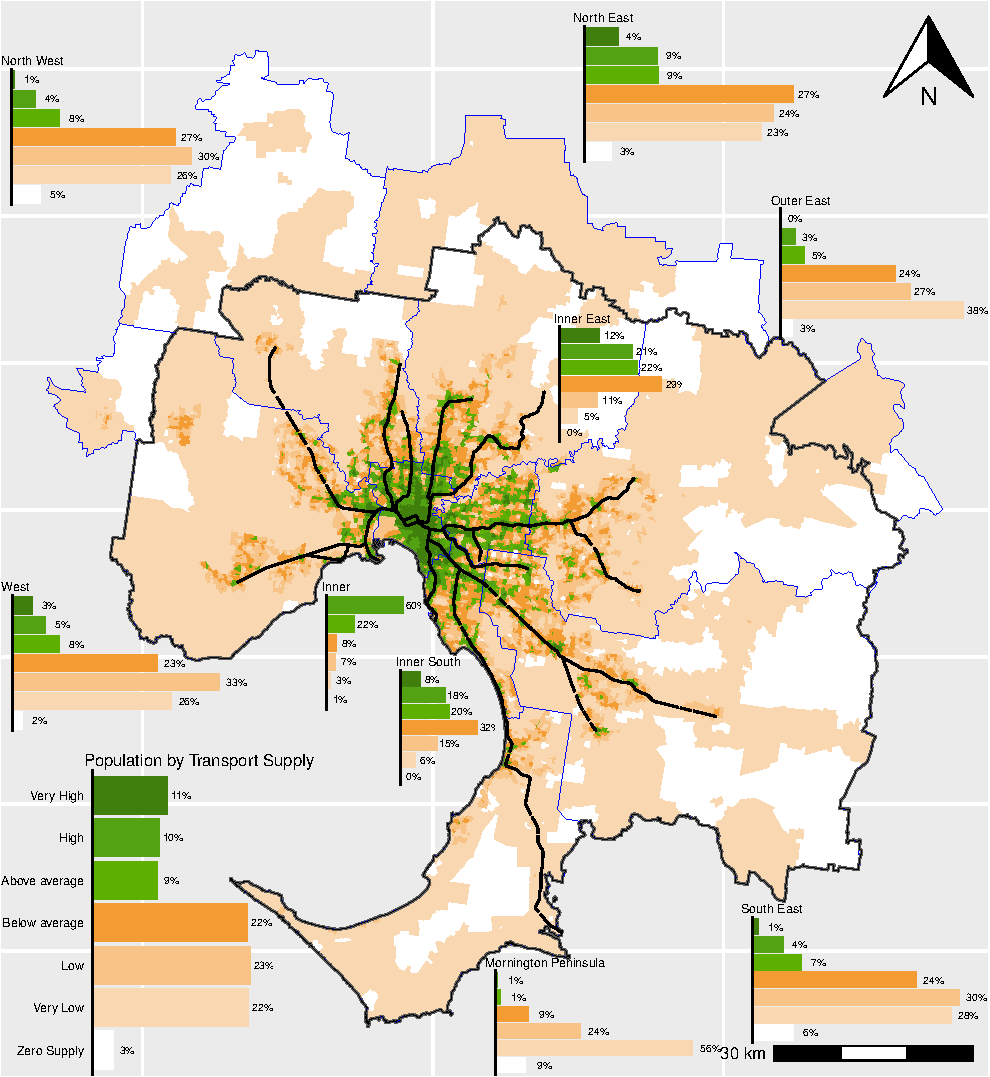
\includegraphics{ReynoldsCurrieQu2024_files/figure-latex/Greater_Melbourne_SA12016_plot_appendix-1.pdf}
\caption{Greater Melbourne, Transit Supply by SA1 for the week starting
the date of the 2016 census, overlayed with: 2006 Greater Melbourne
boundary (black); 2021 SA4 boundaries (blue); and suburban railway lines
(black)}
\end{figure}

\begingroup\fontsize{8}{10}\selectfont

\begin{longtable}[t]{>{\raggedright\arraybackslash}p{1.75cm}>{\raggedleft\arraybackslash}p{1cm}>{\raggedleft\arraybackslash}p{1cm}>{\raggedleft\arraybackslash}p{1cm}>{\raggedleft\arraybackslash}p{1cm}>{\raggedleft\arraybackslash}p{1cm}>{\raggedleft\arraybackslash}p{1cm}>{\raggedleft\arraybackslash}p{1cm}>{\raggedright\arraybackslash}p{1cm}>{\raggedleft\arraybackslash}p{1cm}>{\raggedleft\arraybackslash}p{1.25cm}}
\caption{\label{tab:Greater_Melbourne_SA1_2021_by_SA4}Greater Melbourne 2016: SA1s in each Transport Supply category by SA4}\\
\toprule
Transport Supply & Inner & Inner East & Inner South & North East & North West & Outer East & South East & West & M'ton Pen. & Total\\
\midrule
Zero Supply & 0.0\%     (0) & 0.0\%   (1) & 0.0\%   (5) & 0.6\%    (71) & 0.5\%  (55) & 0.4\%    (44) & 1.2\%   (142) & 1.0\%   (112) & 0.5\%  (59) & 4.3\%    (489)\\
Very Low & 0.1\%    (13) & 0.5\%  (54) & 0.5\%  (63) & 2.7\%   (307) & 2.2\% (254) & 4.6\%   (523) & 5.0\%   (576) & 4.4\%   (504) & 3.5\% (398) & 23.4\%  (2,692)\\
Low & 0.4\%    (48) & 0.9\% (108) & 1.3\% (147) & 2.8\%   (322) & 2.4\% (279) & 3.2\%   (368) & 5.3\%   (608) & 5.7\%   (653) & 1.4\% (158) & 23.4\%  (2,691)\\
Below average & 1.1\%   (130) & 2.7\% (310) & 2.9\% (333) & 3.2\%   (363) & 2.6\% (297) & 2.3\%   (261) & 4.1\%   (470) & 3.8\%   (437) & 0.8\%  (90) & 23.4\%  (2,691)\\
Above average & 1.2\%   (137) & 1.4\% (160) & 1.8\% (210) & 0.9\%   (101) & 0.5\%  (63) & 0.4\%    (49) & 1.0\%   (114) & 1.1\%   (128) & 0.1\%  (13) & 8.5\%    (975)\\
\addlinespace
High & 3.0\%   (345) & 1.5\% (172) & 1.4\% (161) & 0.8\%    (95) & 0.2\%  (22) & 0.3\%    (29) & 0.5\%    (55) & 0.8\%    (93) & 0.0\%   (2) & 8.5\%    (974)\\
Very High & 6.6\%   (763) & 0.6\%  (65) & 0.5\%  (57) & 0.2\%    (26) & 0.0\%   (5) & 0.0\%     (0) & 0.2\%    (19) & 0.3\%    (40) & 0.0\%   (0) & 8.5\%    (975)\\
Total & 12.5\% (1,436) & 7.6\% (870) & 8.5\% (976) & 11.2\% (1,285) & 8.5\% (975) & 11.1\% (1,274) & 17.3\% (1,984) & 17.1\% (1,967) & 6.3\% (720) & 100.0\% (11,487)\\
\bottomrule
\end{longtable}
\endgroup{}

\begingroup\fontsize{8}{10}\selectfont

\begin{longtable}[t]{>{\raggedright\arraybackslash}p{1.75cm}>{\raggedleft\arraybackslash}p{1cm}>{\raggedleft\arraybackslash}p{1cm}>{\raggedleft\arraybackslash}p{1cm}>{\raggedleft\arraybackslash}p{1cm}>{\raggedleft\arraybackslash}p{1cm}>{\raggedleft\arraybackslash}p{1cm}>{\raggedleft\arraybackslash}p{1cm}>{\raggedright\arraybackslash}p{1cm}>{\raggedleft\arraybackslash}p{1cm}>{\raggedleft\arraybackslash}p{1.25cm}}
\caption{\label{tab:Greater_Melbourne_2016_2021_ratio_SA1_table}Greater Melbourne: Share of 2021 SA1s by change in transit service (2016 vs 2021) by SA4 region}\\
\toprule
Change & Inner & Inner East & Inner South & North East & North West & Outer East & South East & West & M'ton Pen. & Total\\
\midrule
New service & 0.0\%     (0) & 0.0\%   (0) & 0.0\%   (0) & 0.2\%    (20) & 0.7\%  (79) & 0.0\%     (1) & 1.0\%   (113) & 0.8\%    (87) & 0.1\%   (6) & 2.7\%    (306)\\
Increased 30\% or more & 0.0\%     (5) & 0.0\%   (1) & 0.7\%  (83) & 0.9\%   (107) & 1.5\% (173) & 0.1\%    (10) & 2.6\%   (293) & 2.5\%   (290) & 1.3\% (154) & 9.7\%  (1,116)\\
Increased 10 to 30\% & 0.9\%   (104) & 0.1\%   (7) & 0.9\%  (99) & 0.8\%    (95) & 1.2\% (133) & 0.5\%    (54) & 1.5\%   (173) & 2.0\%   (231) & 0.4\%  (49) & 8.2\%    (945)\\
Increased 5 to 10\% & 1.4\%   (166) & 0.2\%  (28) & 1.0\% (120) & 0.8\%    (90) & 0.7\%  (75) & 0.6\%    (69) & 1.0\%   (120) & 2.0\%   (233) & 0.2\%  (23) & 8.0\%    (924)\\
Increased 3 to 5\% & 1.6\%   (185) & 0.5\%  (58) & 0.6\%  (71) & 1.3\%   (147) & 1.1\% (122) & 0.5\%    (63) & 0.9\%   (104) & 1.8\%   (210) & 0.3\%  (32) & 8.6\%    (992)\\
\addlinespace
Increased 1 to 3\% & 2.4\%   (281) & 1.3\% (152) & 1.2\% (142) & 1.9\%   (214) & 0.9\% (107) & 0.9\%   (101) & 1.5\%   (176) & 2.4\%   (271) & 0.7\%  (76) & 13.2\%  (1,520)\\
Within 1\% & 2.5\%   (286) & 3.9\% (444) & 1.9\% (223) & 2.6\%   (295) & 1.2\% (138) & 5.8\%   (661) & 5.4\%   (620) & 3.0\%   (347) & 2.3\% (261) & 28.5\%  (3,275)\\
Reduced 1 to 3\% & 1.0\%   (114) & 0.8\%  (94) & 0.5\%  (63) & 0.8\%    (89) & 0.3\%  (32) & 0.8\%    (92) & 0.7\%    (77) & 0.4\%    (44) & 0.4\%  (42) & 5.6\%    (647)\\
Reduced 3 to 10\% & 1.8\%   (212) & 0.5\%  (61) & 0.9\% (100) & 0.9\%   (105) & 0.2\%  (28) & 0.9\%   (102) & 0.5\%    (58) & 0.7\%    (79) & 0.1\%  (15) & 6.6\%    (760)\\
Reduced 10\% or more & 0.7\%    (83) & 0.2\%  (24) & 0.6\%  (70) & 0.5\%    (52) & 0.3\%  (33) & 0.7\%    (77) & 0.9\%   (108) & 0.5\%    (63) & 0.0\%   (3) & 4.5\%    (513)\\
\addlinespace
Service withdrawn (magenta) & 0.0\%     (0) & 0.0\%   (0) & 0.0\%   (0) & 0.0\%     (4) & 0.0\%   (1) & 0.0\%     (3) & 0.0\%     (3) & 0.0\%     (4) & 0.0\%   (0) & 0.1\%     (15)\\
Never served (black) & 0.0\%     (0) & 0.0\%   (1) & 0.0\%   (5) & 0.6\%    (67) & 0.5\%  (54) & 0.4\%    (41) & 1.2\%   (139) & 0.9\%   (108) & 0.5\%  (59) & 4.1\%    (474)\\
Total & 12.5\% (1,436) & 7.6\% (870) & 8.5\% (976) & 11.2\% (1,285) & 8.5\% (975) & 11.1\% (1,274) & 17.3\% (1,984) & 17.1\% (1,967) & 6.3\% (720) & 100.0\% (11,487)\\
\bottomrule
\end{longtable}
\endgroup{}

\begin{figure}
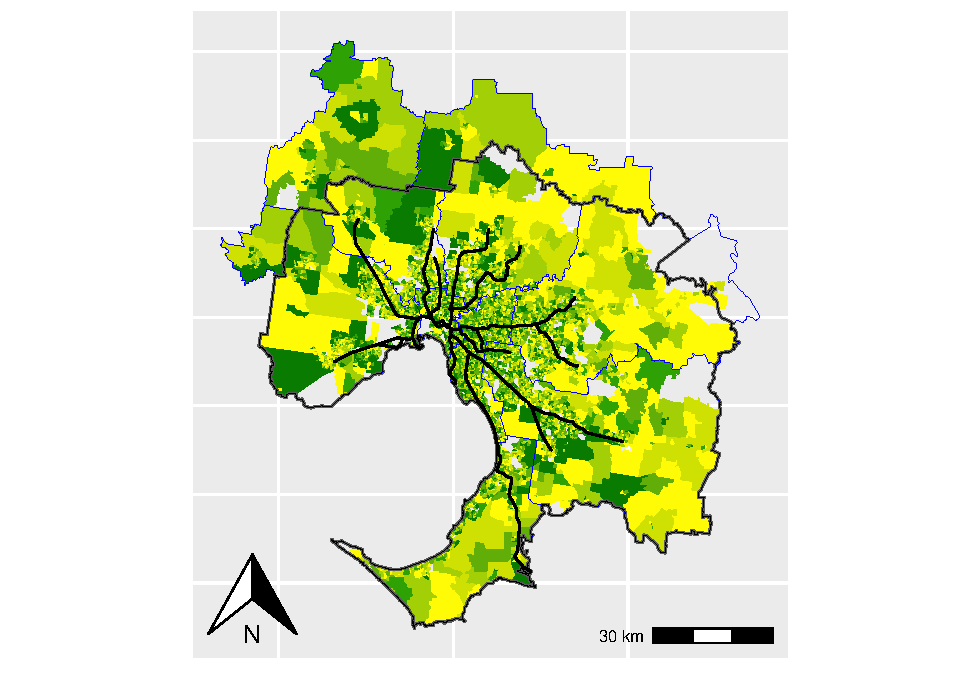
\includegraphics[width=0.9\linewidth]{ReynoldsCurrieQu2024_files/figure-latex/Greater_Melbourne_2016_social_needs_appendix-1} \caption{Distribution of categories of composite social need index scores in 2016 (left) and 2021 (right), overlayed with: 2006 Greater Melbourne boundary (black); middle/outer and inner/middle suburb boundaries (grey); and suburban railway lines (dashed).}\label{fig:Greater_Melbourne_2016_social_needs_appendix-1}
\end{figure}
\begin{figure}
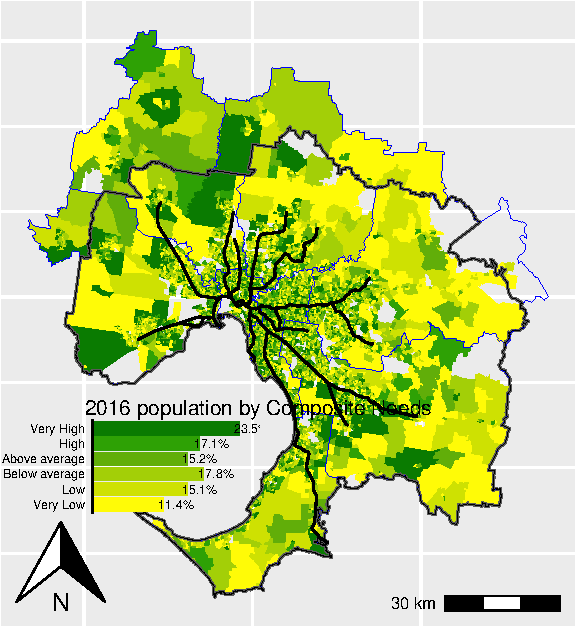
\includegraphics[width=0.9\linewidth]{ReynoldsCurrieQu2024_files/figure-latex/Greater_Melbourne_2016_social_needs_appendix-2} \caption{Distribution of categories of composite social need index scores in 2016 (left) and 2021 (right), overlayed with: 2006 Greater Melbourne boundary (black); middle/outer and inner/middle suburb boundaries (grey); and suburban railway lines (dashed).}\label{fig:Greater_Melbourne_2016_social_needs_appendix-2}
\end{figure}

Figure \ref{fig:Greater_Melbourne_2016_social_needs_appendix} shows the
spatial patterns of social needs in 2016. Compared to 2021, the spatial
patterns appear similar, with some areas in the north-west (Gisborne)
and south-east (Carrum Downs, Stoney Point) having Very High needs in
both. Some caution may be required in making direct comparisons of many
outer suburbs where residential development has led to the introduction
of new SA1s for the 2021 census. In many areas, including in the
south-west (Werribee), north-west (Romsey), north (Wallan, Beveridge,
Mickleham) and south-east (Clyde North and Beaconsfield South), it
appears there are still Very High transport needs but the spatial area
covered on the map is much smaller due to the redistricting of larger
SA1s into multiple SA1s. That said, it appears that:

\begin{itemize}
\tightlist
\item
  social needs fell in the southern parts of Bacchus Marsh and areas
  around Melton (outer west);
\item
  social needs rose in some outer northern (Lancefield), eastern
  (Gembrook East) and southern (end of the Mornington Penninsula) areas.
\end{itemize}

\begin{figure}
\centering
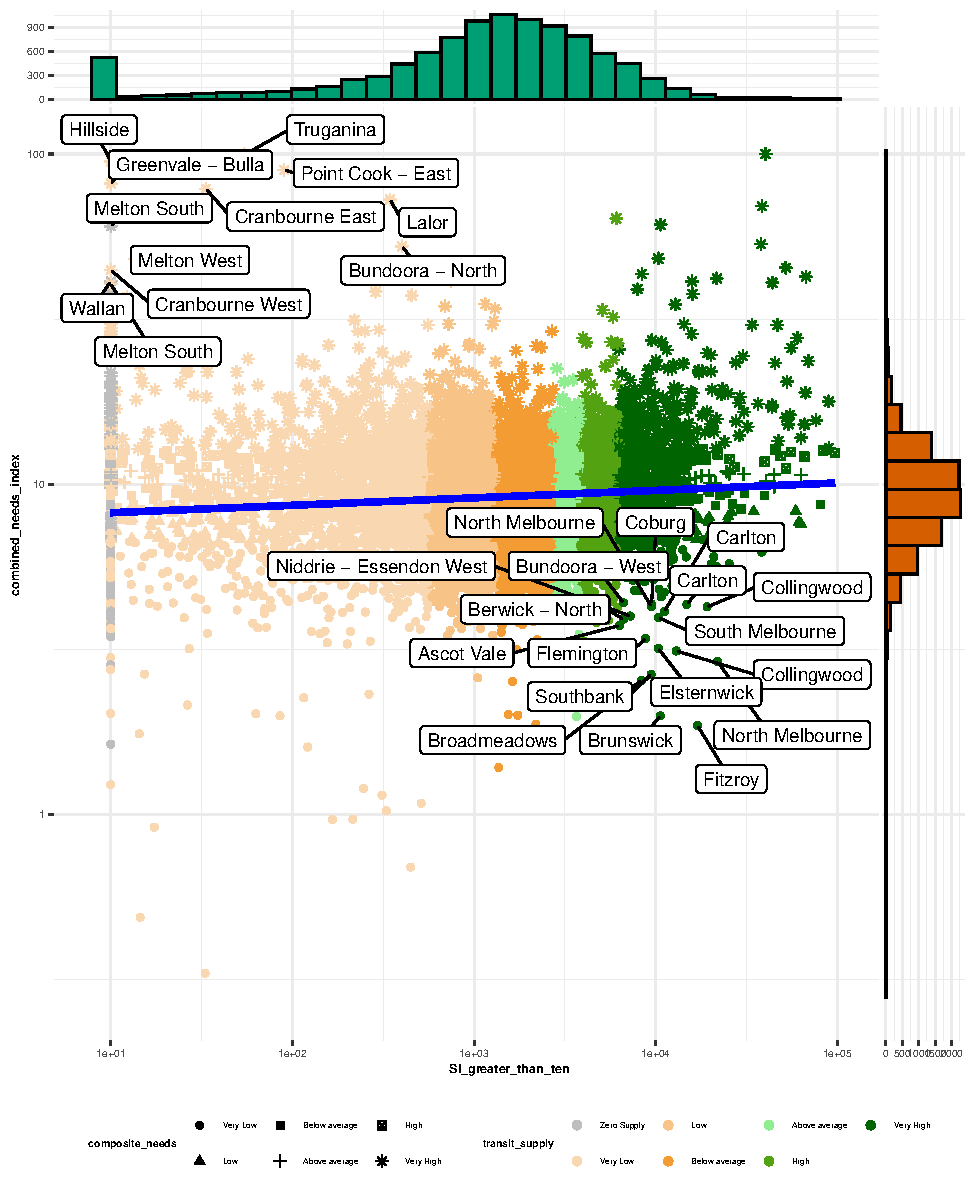
\includegraphics{ReynoldsCurrieQu2024_files/figure-latex/Greater_Melbourne_2016_needs_gap_scatterplot_figure-1.pdf}
\caption{Greater Melbourne 2016, SI and Combined Needs Index scores,
with SI scores \textless{} 10 rounded up to equal 10.}
\end{figure}

\bibliography{References.bib, packages.bib}


\end{document}
